\documentclass[10pt]{article}
\usepackage[margin=1in]{geometry}
 \usepackage{auto-pst-pdf}
\usepackage{graphicx}
%\usepackage{arydshln}
\usepackage{ifpdf}
\ifpdf
  \usepackage{epstopdf}
\fi
\usepackage{multirow}
\usepackage{epsfig}
\usepackage{float}
\usepackage{url}
\usepackage{color}
\usepackage{subfigure}

%\newcommand\solidrule[1][1cm]{\rule[0.5ex]{#1}{.4pt}}
%\newcommand\dashedrule{\mbox{%
%  \solidrule[2mm]\hspace{2mm}\solidrule[2mm]\hspace{2mm}\solidrule[2mm]}}
  
%\usepackage{hyperref}

\begin{document}
\title{Empirical Check of Machine Homogeneity on Timing Protocol}

\author{
Young-Kyoon Suh\\
Data-Intensive Systems Laboratory\\
School of Computer Science and Engineering\\
Kyungpook National University\\
}
\maketitle

\section{Description}
In this work we do a check to see if the result on the same experiment is different 
on different nodes, each with the same machine specification.

\section{Preliminary Experiments}

We provide a short description of our preliminary experimental runs. 

\paragraph{Experimental Notes:} In our experiments 
we used four nodes ({\tt sodb8}, {\tt sodb9}, {\tt sodb10}, and {\tt sodb12} ) in the same cluster. 
A short summary of the experiments is exhibited in Table~\ref{tab:exp_notes}.

%% done
\begin{table}[h]
\begin{center}
\begin{tabular}{|p{4cm}|p{3cm}|p{4cm}|p{4cm}|} \hline
Machine & Task Length & Description & Time Length\\ \hline
{\tt sodb8} (plugged into {\em bottom left} power strip) & INC1$\sim$INC128 & Runs of 300 samples & 2017-02-09 $\sim$ 2017-02-10\\ \hline
{\tt sodb9}  (plugged into {\em the upper left} power strip)  &  INC1$\sim$INC128 & Runs of 300 samples & 2017-02-09 $\sim$ 2017-02-10\\ \hline
{\tt sodb10}  (plugged into {\em the upper left} power strip)  & INC1$\sim$INC128 & Runs of 300 samples & 2017-02-09 $\sim$ 2017-02-10\\ \hline
{\tt sodb12}  (plugged into {\em the upper left} power strip)  & INC1$\sim$INC128 & Runs of 300 samples & 2017-02-09 $\sim$ 2017-02-10\\ \hline
\end{tabular}
\end{center}
\vspace{-.2in}
\caption{Detailed description of INC data used for histograms\label{tab:exp_notes}}
\end{table}

\clearpage
\newpage
\paragraph{Measurement Quality Across the SoDB Nodes:} 
Fig.~\ref{fig:machine_comp} shows 
the standard deviation and relative error of 
elapsed time (ET) and process time (PT) on the different SoDB nodes 
as the task length of INC increases. 

\begin{figure}[h]
	\centering
	\subfigure[Standard Deviation - ET]{
		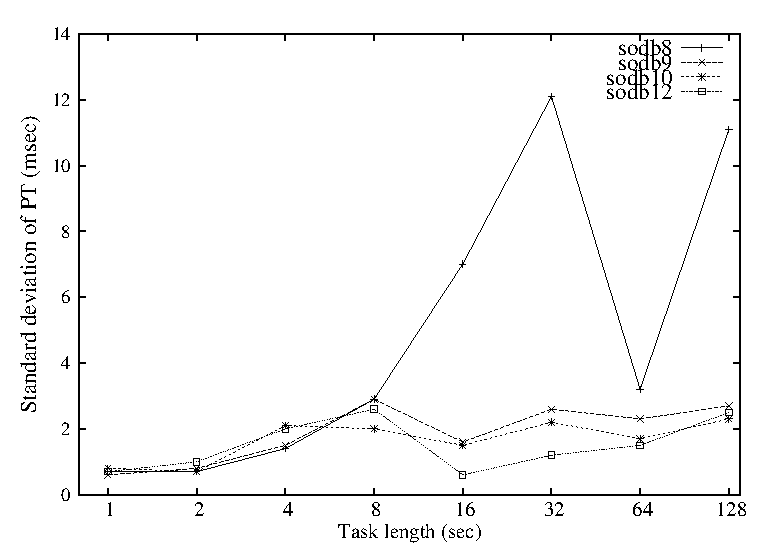
\includegraphics[scale=0.6]{overall/machine_et_std.eps}
        \label{fig:et_std}
    }
    \subfigure[Relative Error - ET]{
        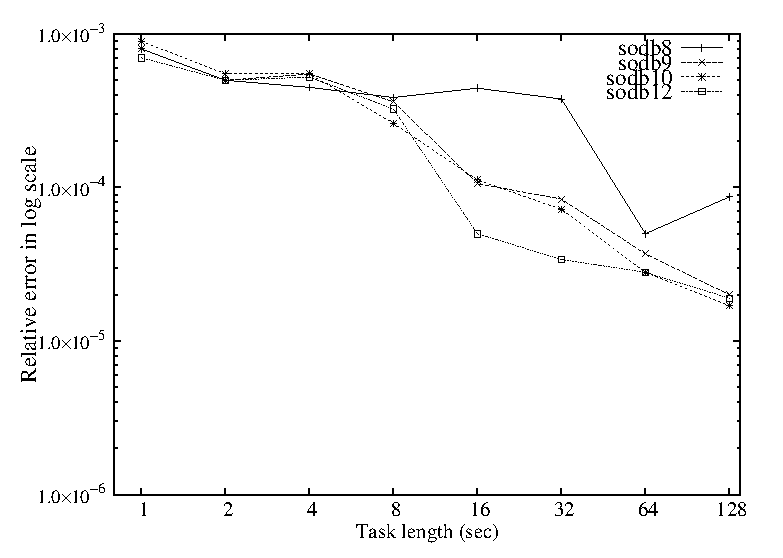
\includegraphics[scale=0.6]{overall/machine_et_re.eps}
        \label{fig:et_re}
    }
	\subfigure[Standard Deviation - PT]{
		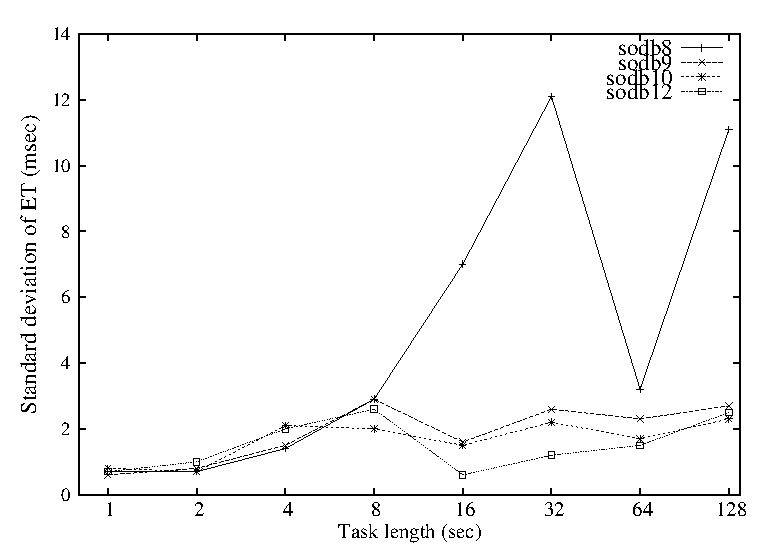
\includegraphics[scale=0.6]{overall/machine_pt_std.eps}
        \label{fig:pt_std}
    }
    \subfigure[Relative Error - PT]{
        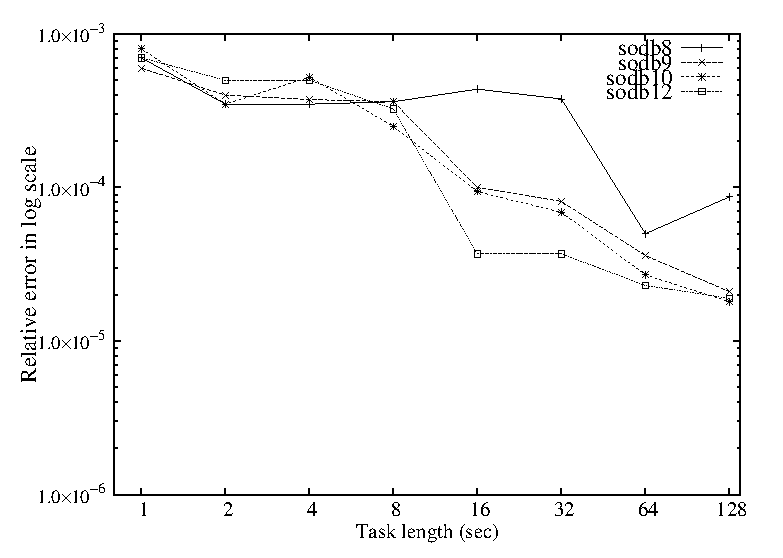
\includegraphics[scale=0.6]{overall/machine_pt_re.eps}
        \label{fig:pt_re}
    }
    \caption{Measurement Quality Comparison among Different SoDB Machines}
    \label{fig:machine_comp}
\end{figure}

%\newpage

Each of the following sections exhibits histograms of ET and PT 
over increasing INC's task lengths on each individual node. 

\newpage

\subsection{{\tt sodb12}~\label{sec:sodb12_hist}} 
This section exhibits histograms on the EMPv5 data obtained on {\tt sodb12}. 
The detailed description of the base data are from Table~\ref{tab:exp_notes}.

\subsubsection{ET}

\begin{figure}[hp!]
	\centering
	\subfigure[ET frequency on INC1 on {\tt sodb12}]{
		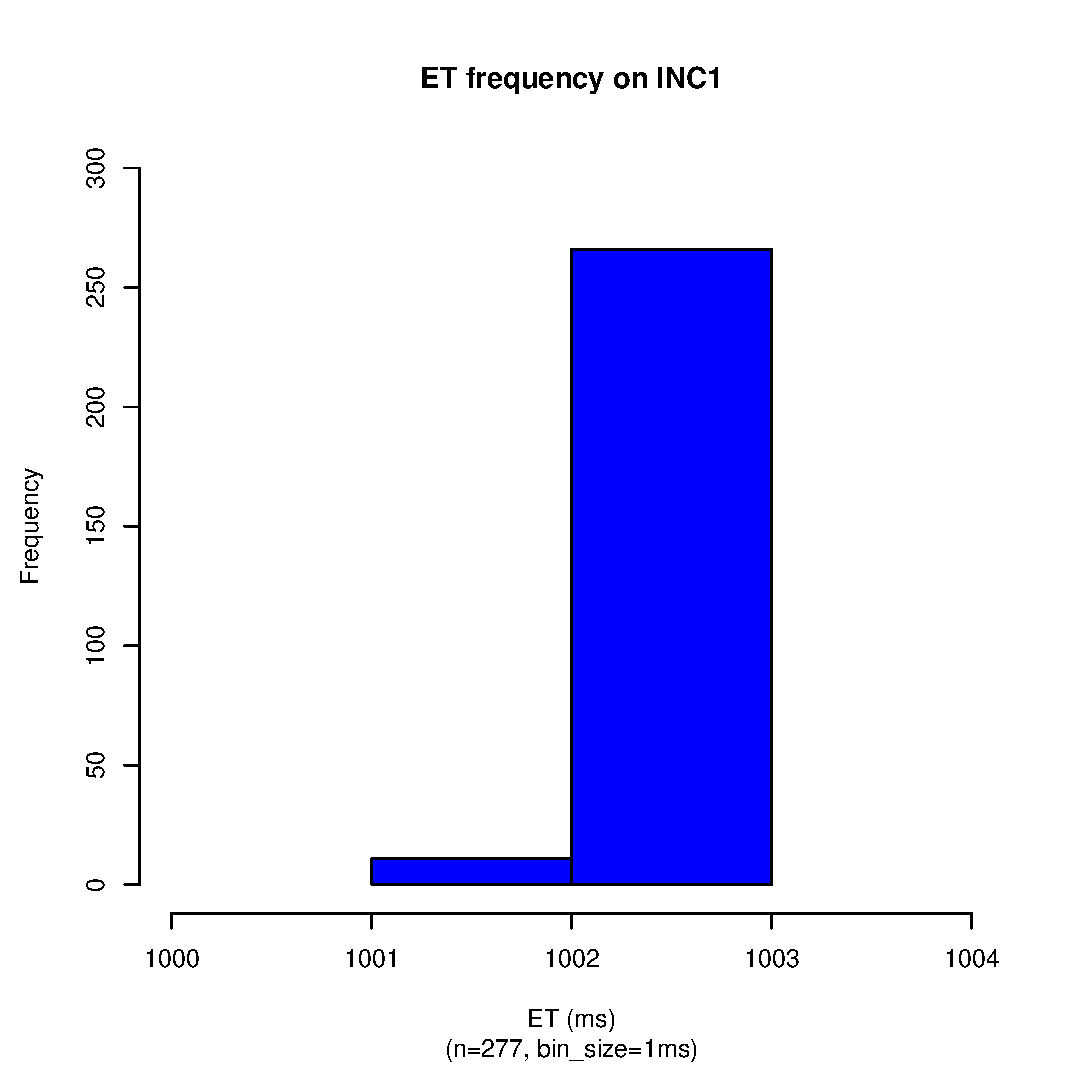
\includegraphics[scale=0.43]{sodb12/1_sec_et_hist_v5.eps}
		\label{fig:s12_inc1_et_hist_v5}
	}
	\subfigure[ET frequency on INC2 on {\tt sodb12}]{
		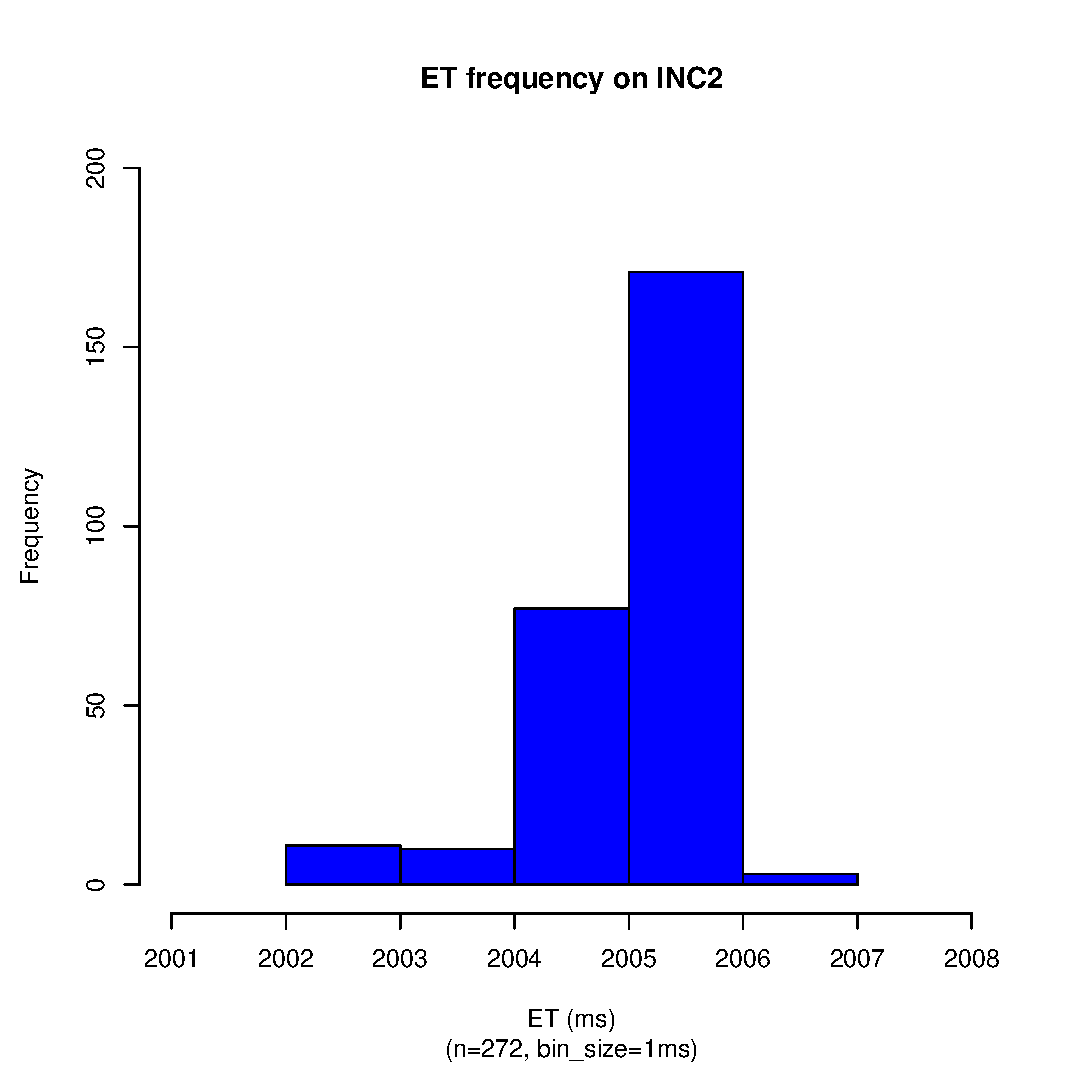
\includegraphics[scale=0.43]{sodb12/2_sec_et_hist_v5.eps}
		\label{fig:s12_inc2_et_hist_v5}
	}
	\subfigure[ET frequency on INC4 on {\tt sodb12}]{
		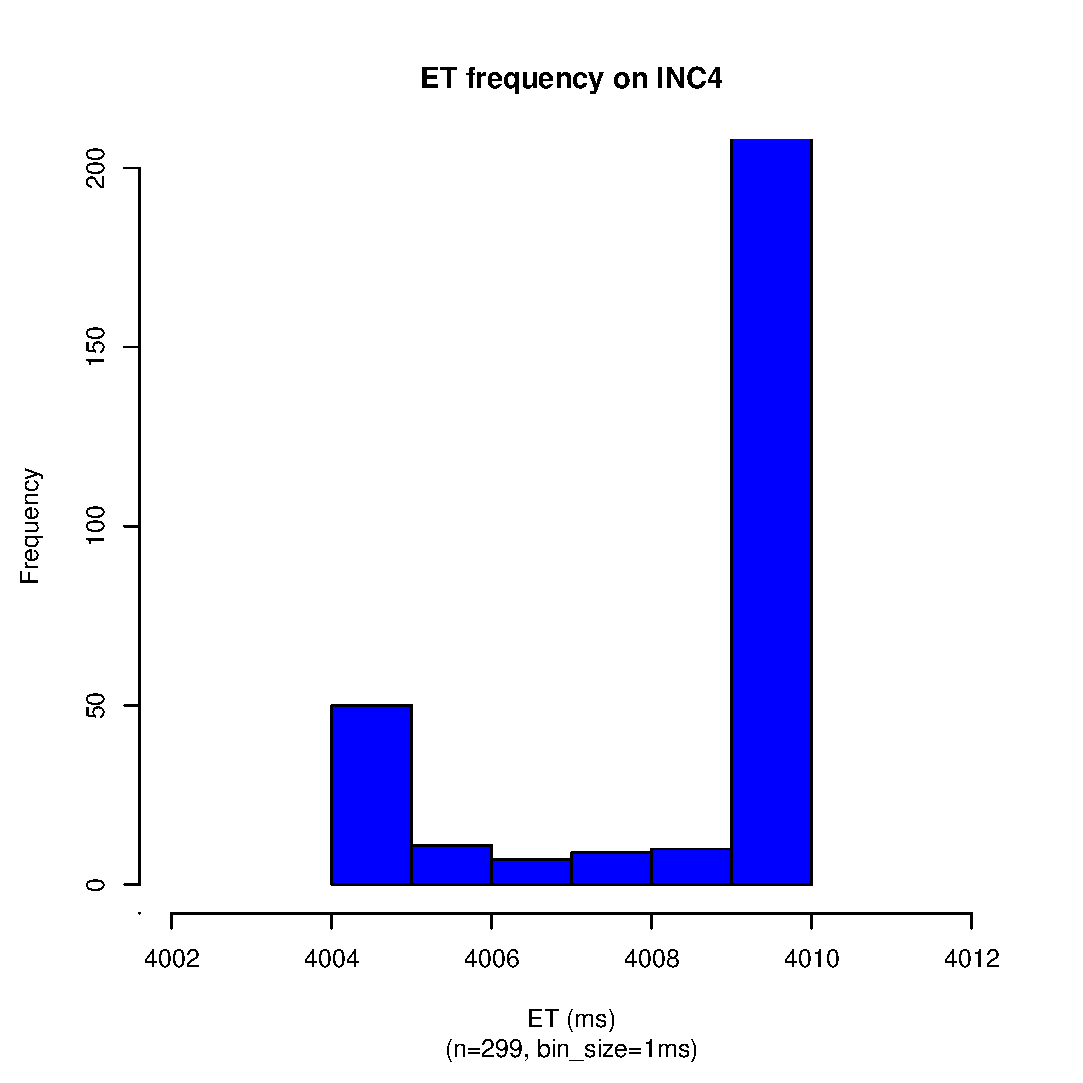
\includegraphics[scale=0.43]{sodb12/4_sec_et_hist_v5.eps}
		\label{fig:s12_inc4_et_hist_v5}
	}
	\subfigure[ET frequency on INC8 on {\tt sodb12}]{
		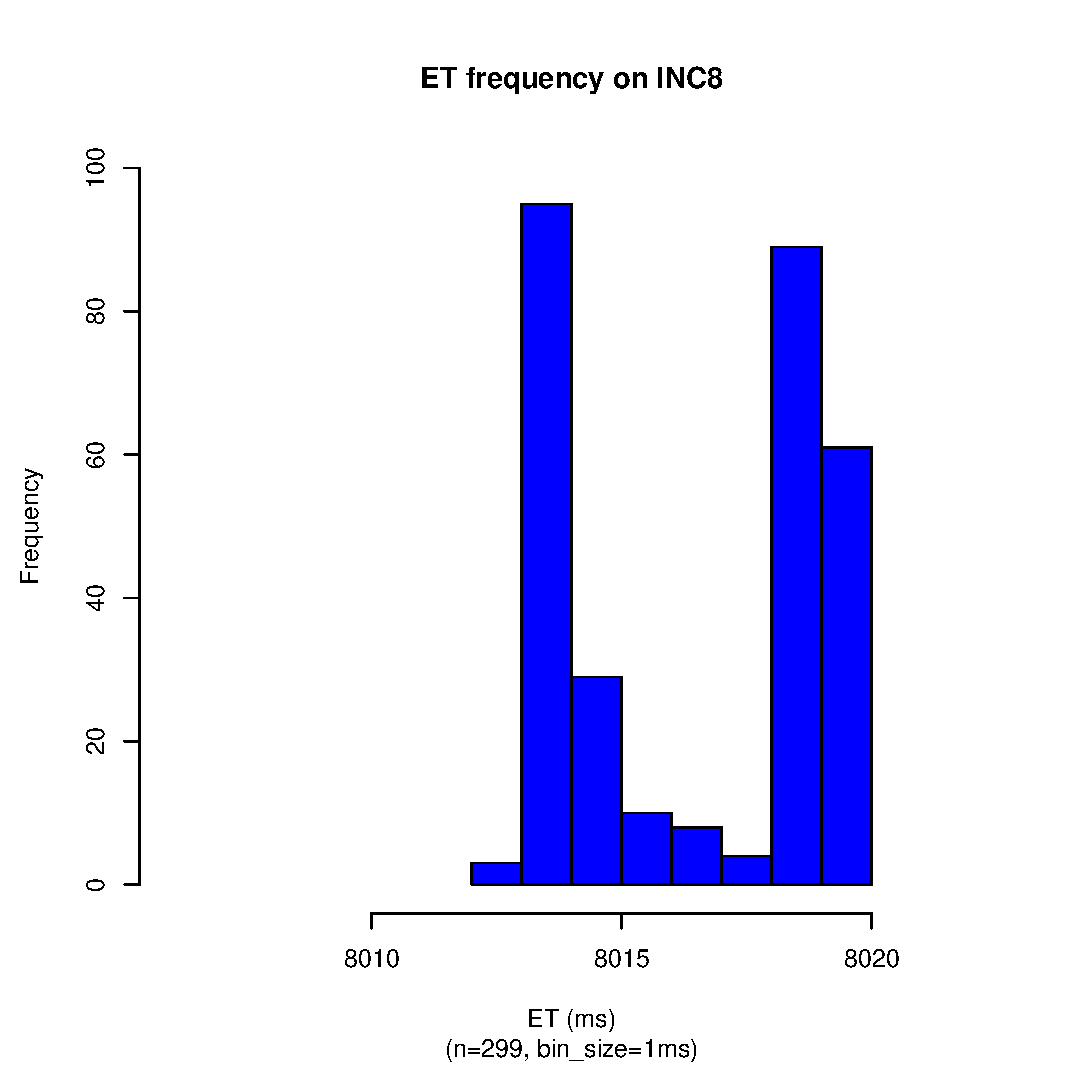
\includegraphics[scale=0.43]{sodb12/8_sec_et_hist_v5.eps}
		\label{fig:s12_inc8_et_hist_v5}
	}
	\caption{ET Histograms of INC1 ... INC8~\label{fig:s12_et_hist1}}
\end{figure}

\begin{figure}[hp!]
	\centering
	\subfigure[ET frequency on INC16 on {\tt sodb12}]{
		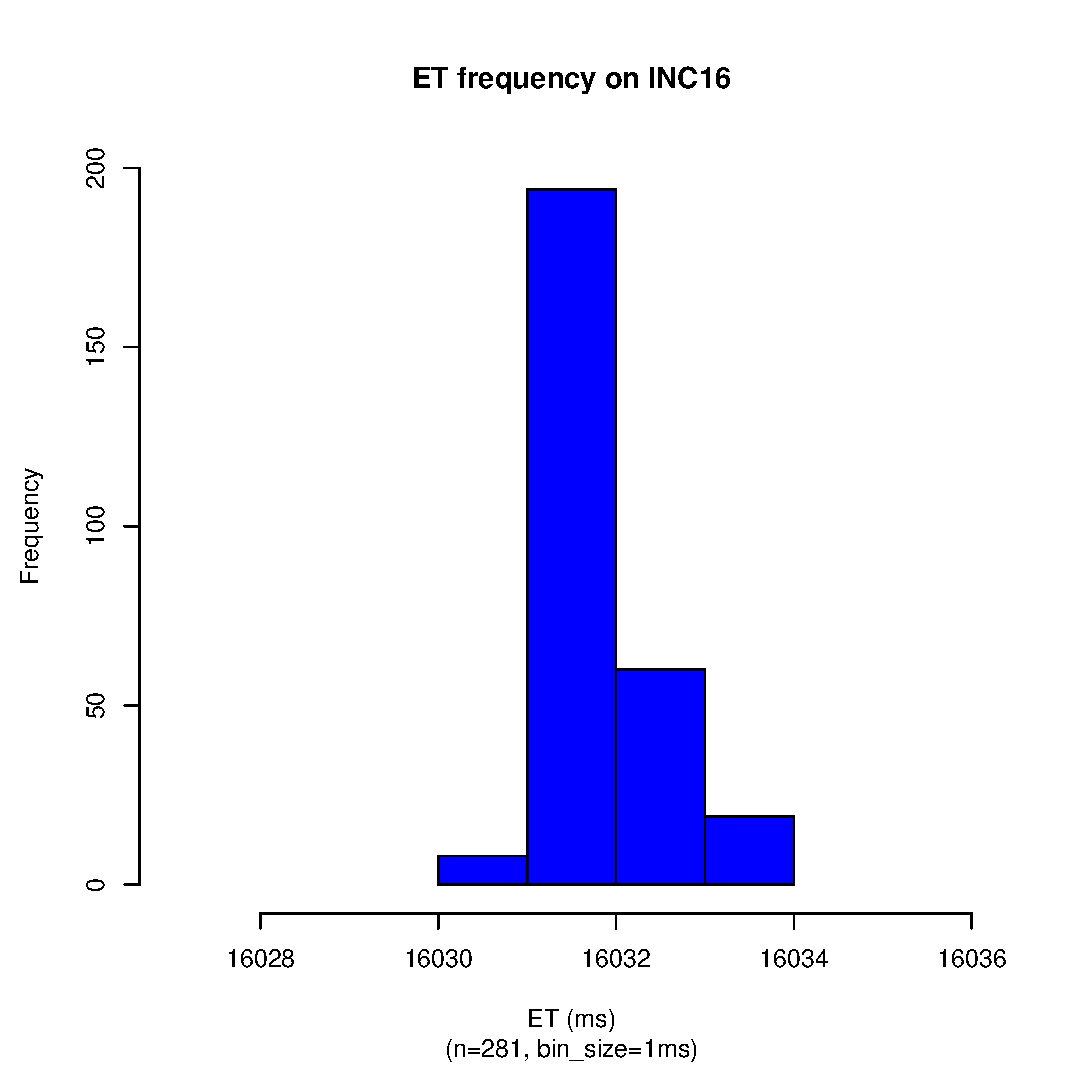
\includegraphics[scale=0.43]{sodb12/16_sec_et_hist_v5.eps}
		\label{fig:s12_inc16_et_hist_v5}
	}
	\subfigure[ET frequency on INC32 on {\tt sodb12}]{
		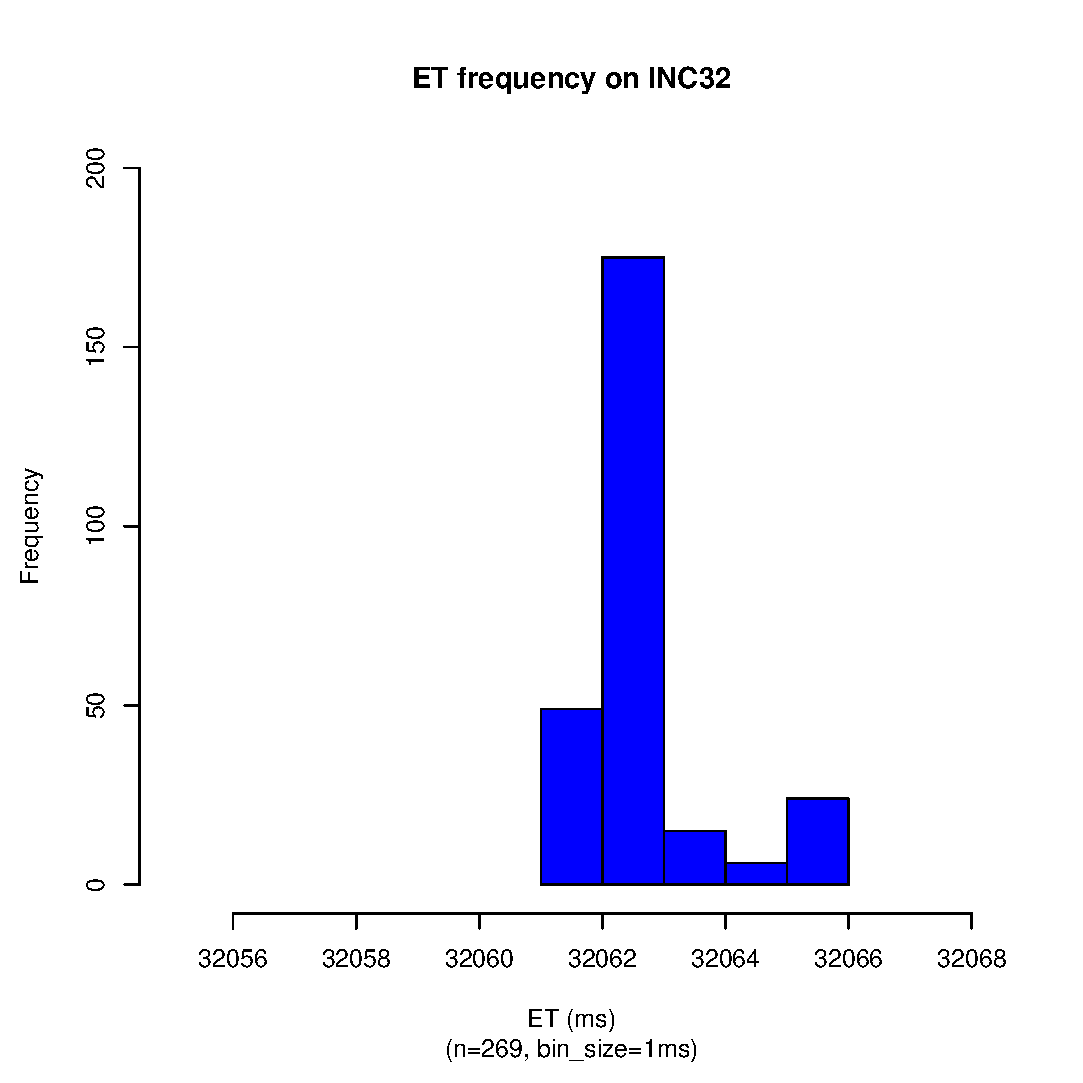
\includegraphics[scale=0.43]{sodb12/32_sec_et_hist_v5.eps}
		\label{fig:s12_inc32_et_hist_v5}
	}
	\subfigure[ET frequency on INC64 on {\tt sodb12}]{
		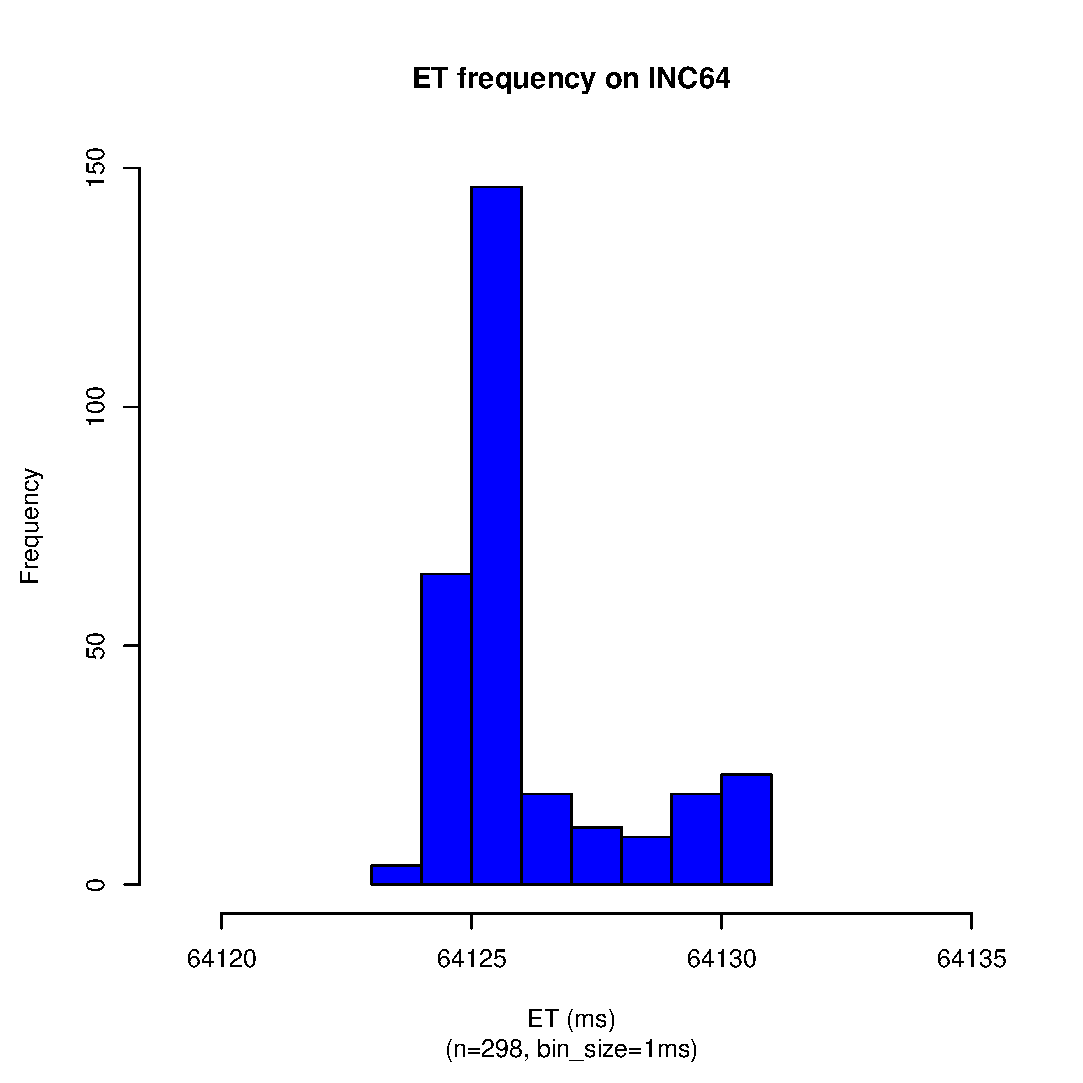
\includegraphics[scale=0.43]{sodb12/64_sec_et_hist_v5.eps}
		\label{fig:s12_inc64_et_hist_v5}
	}
	\subfigure[ET frequency on INC128 on {\tt sodb12}]{
		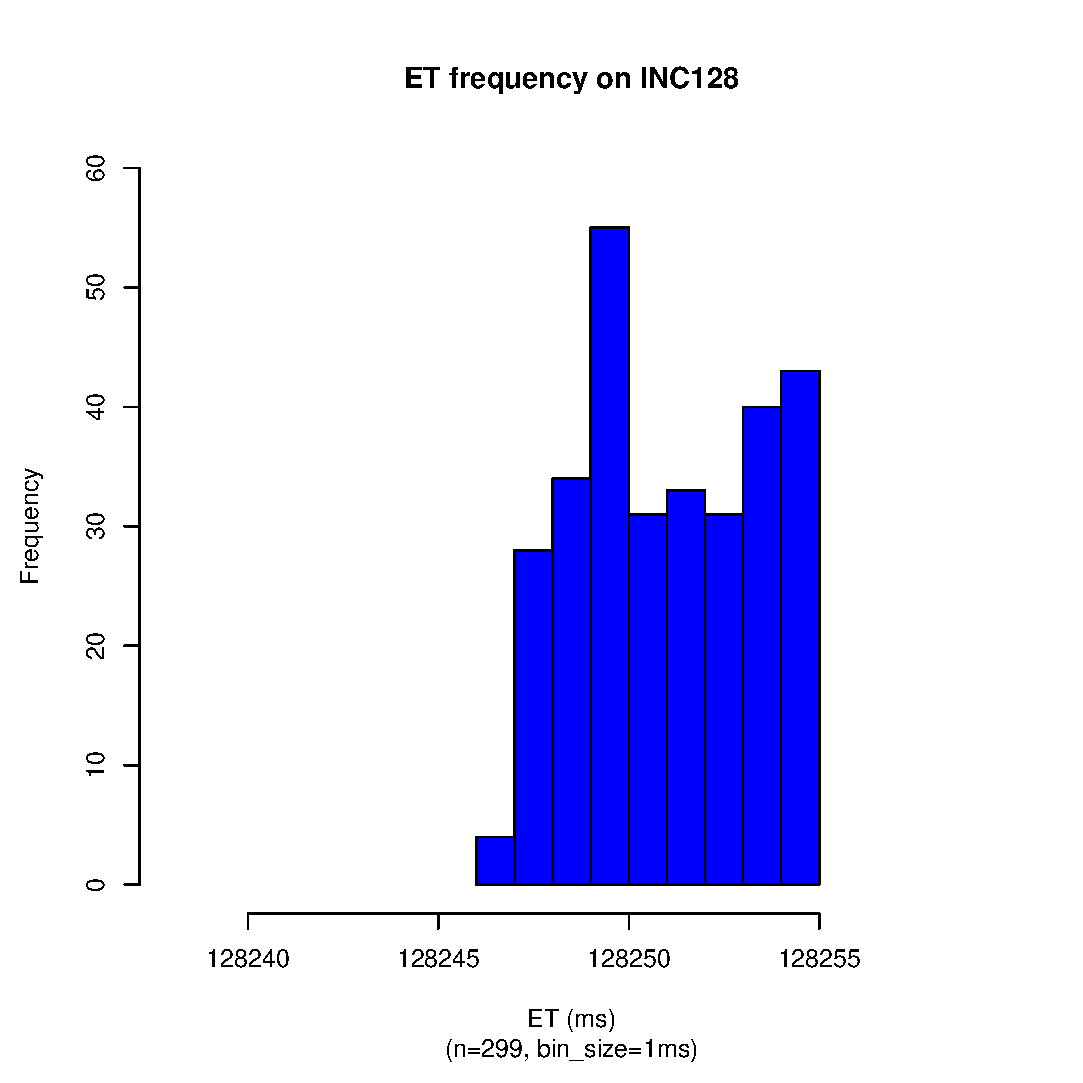
\includegraphics[scale=0.43]{sodb12/128_sec_et_hist_v5.eps}
		\label{fig:s12_inc128_et_hist_v5}
	}
	\caption{ET Histograms of INC16 ... INC128~\label{fig:s12_et_hist2}}
\end{figure}

\newpage

\subsubsection{PT}

\begin{figure}[hp!]
	\centering
	\subfigure[PT frequency on INC1 on {\tt sodb12}]{
		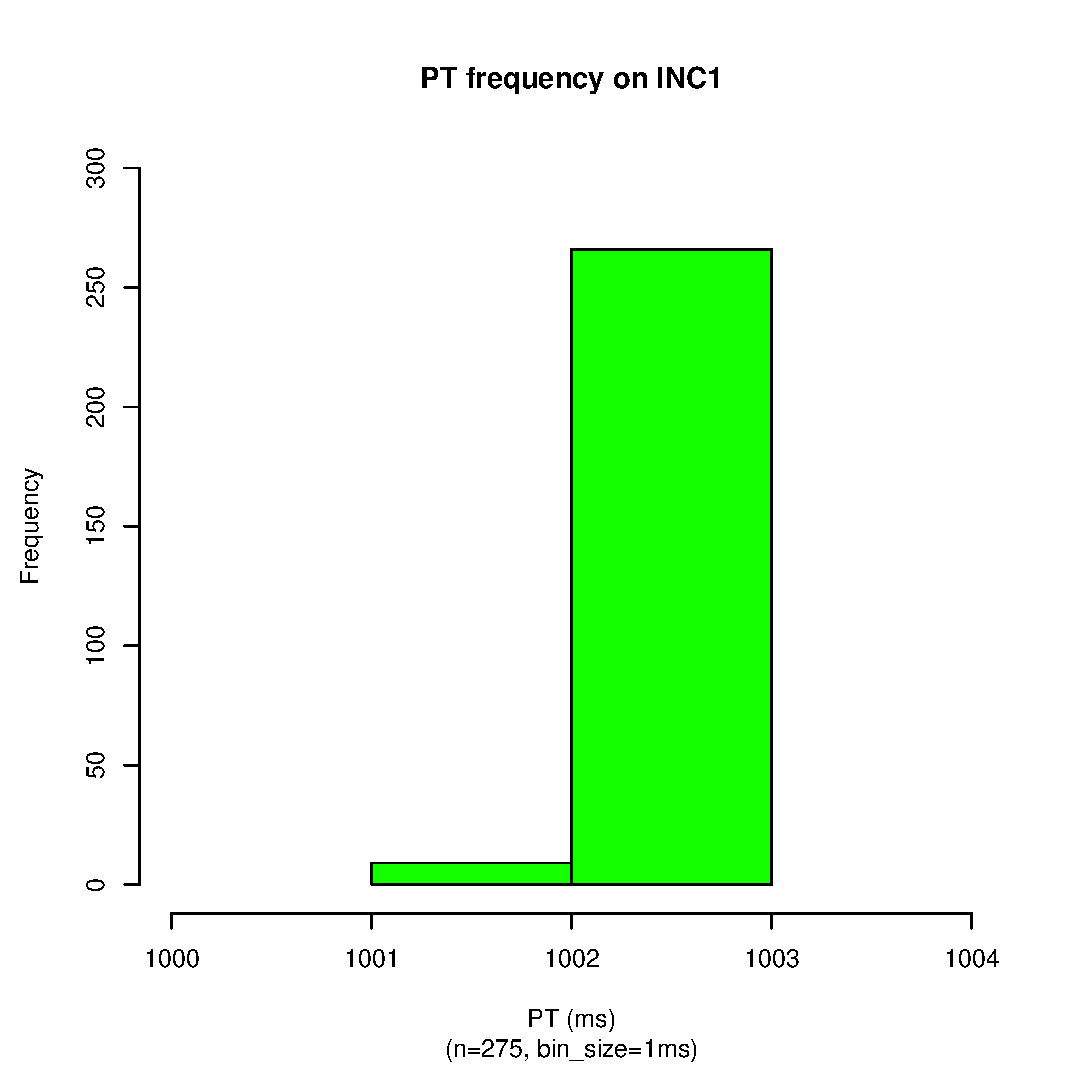
\includegraphics[scale=0.43]{sodb12/1_sec_pt_hist_v5.eps}
		\label{fig:s12_inc1_hist_v5}
	}
	\subfigure[PT frequency on INC2 on {\tt sodb12}]{
		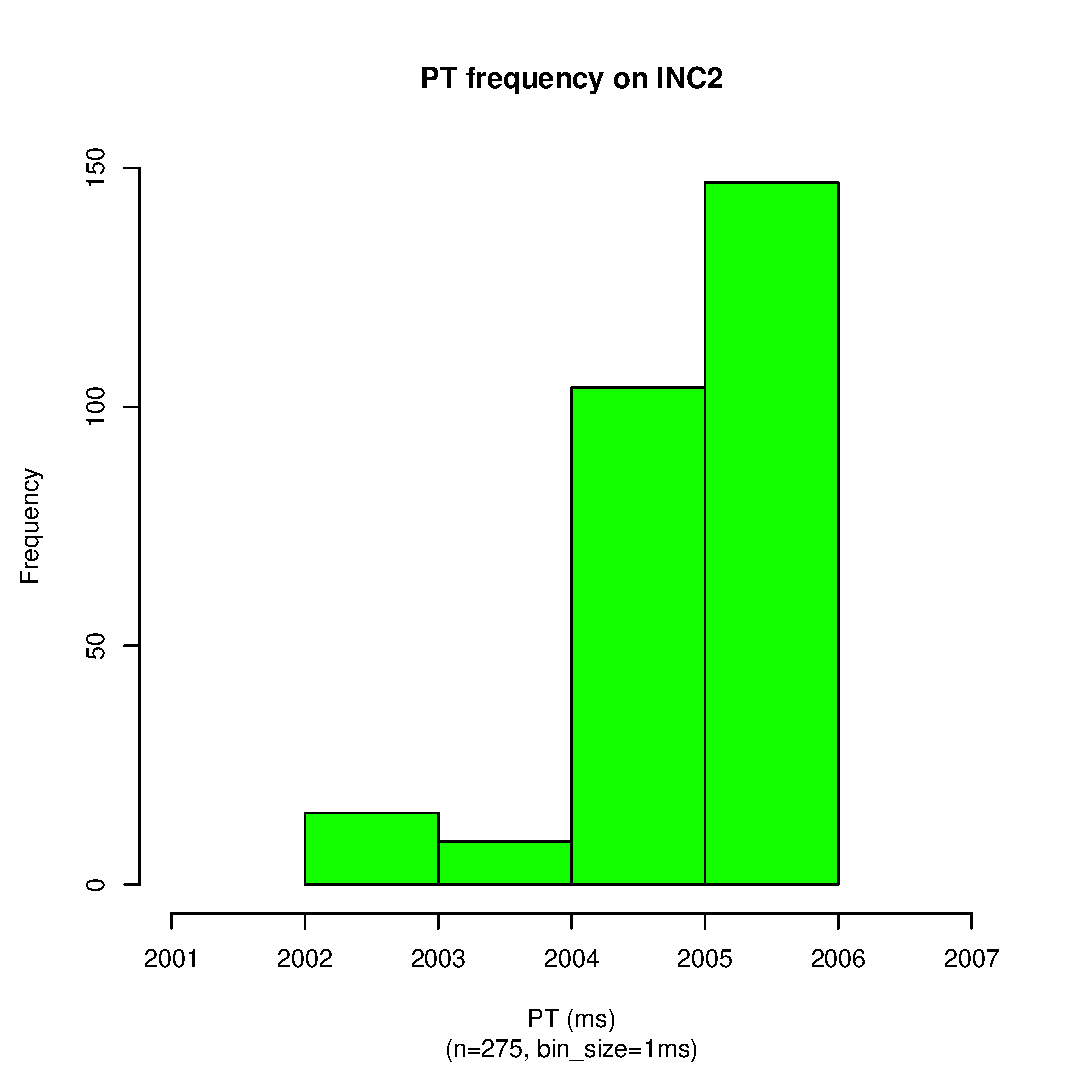
\includegraphics[scale=0.43]{sodb12/2_sec_pt_hist_v5.eps}
		\label{fig:s12_inc2_hist_v5}
	}
	\subfigure[PT frequency on INC4 on {\tt sodb12}]{
		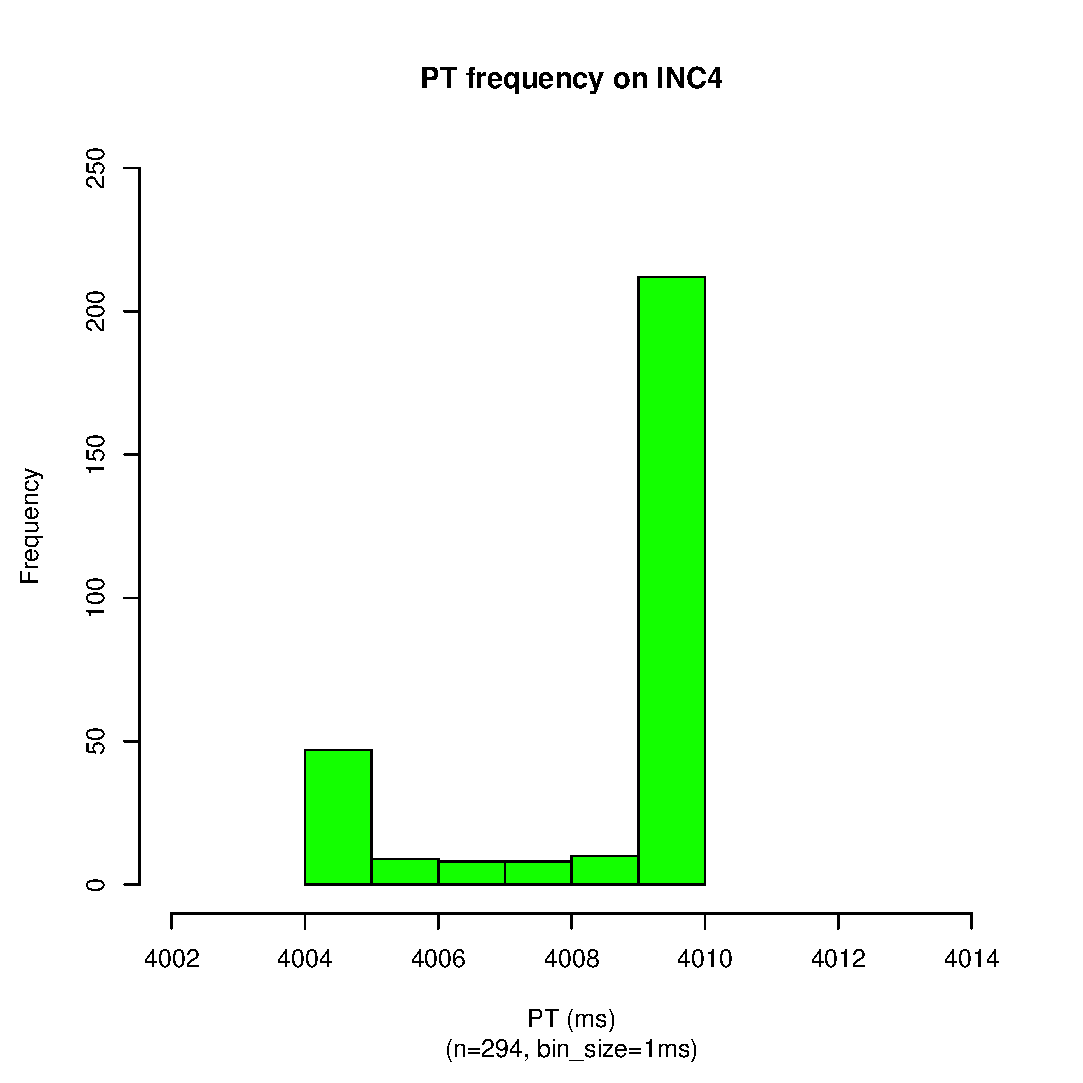
\includegraphics[scale=0.43]{sodb12/4_sec_pt_hist_v5.eps}
		\label{fig:s12_inc4_hist_v5}
	}
	\subfigure[PT frequency on INC8 on {\tt sodb12}]{
		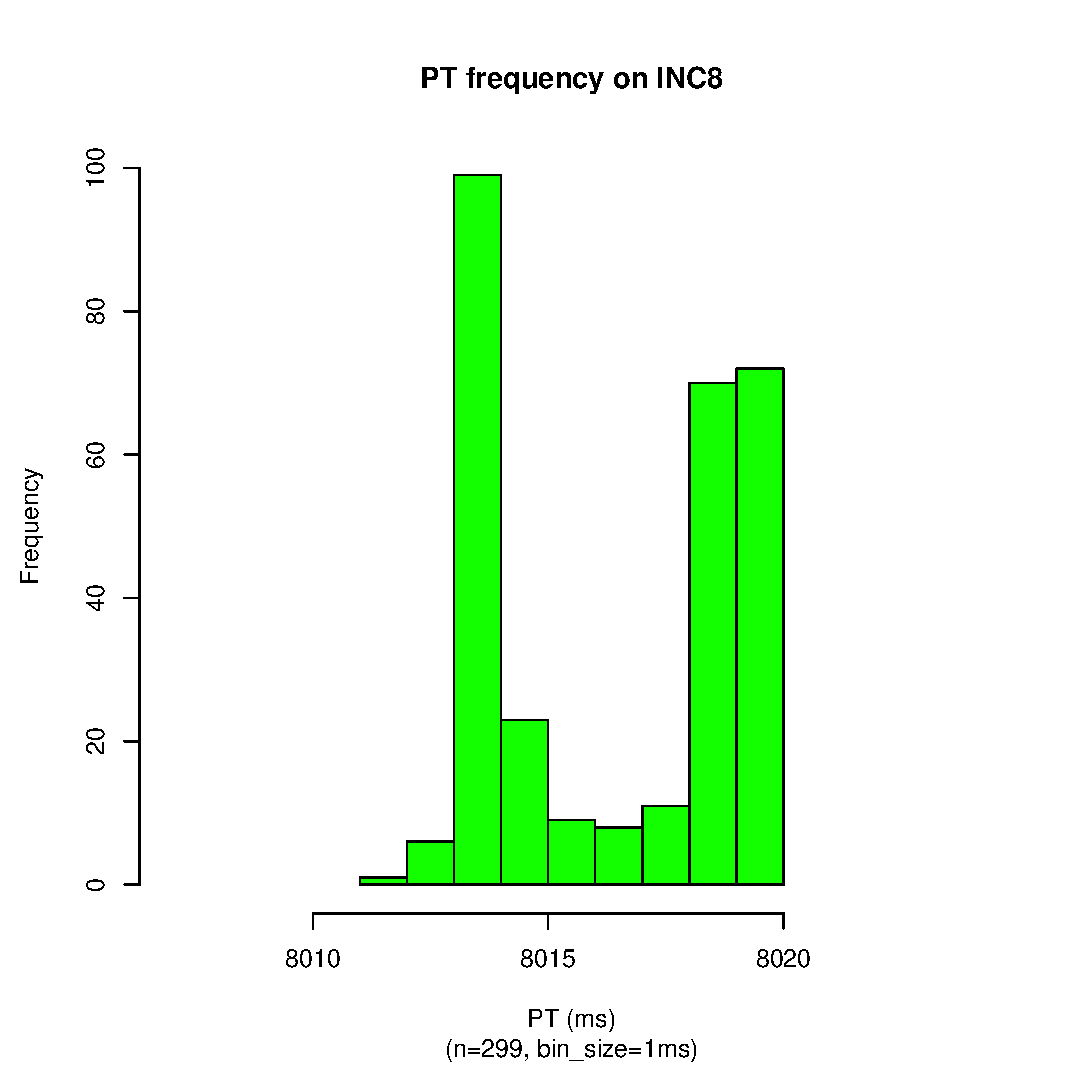
\includegraphics[scale=0.43]{sodb12/8_sec_pt_hist_v5.eps}
		\label{fig:s12_inc8_hist_v5}
	}
	\caption{PT Histograms of INC1 ... INC8~\label{fig:s12_pt_hist1}}
\end{figure}

\begin{figure}[hp!]
	\centering
	\subfigure[PT frequency on INC16 on {\tt sodb12}]{
		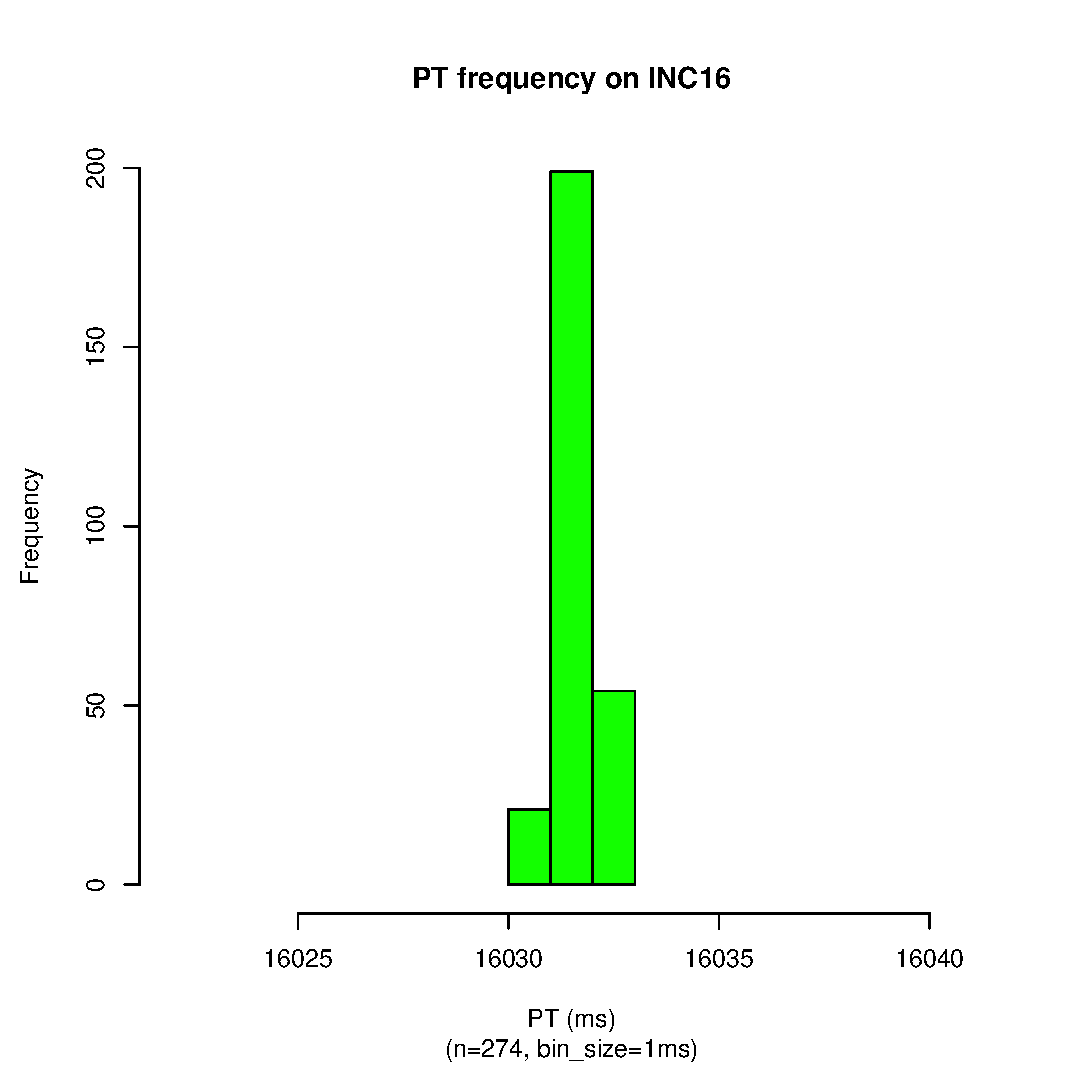
\includegraphics[scale=0.43]{sodb12/16_sec_pt_hist_v5.eps}
		\label{fig:s12_inc16_hist_v5}
	}
	\subfigure[PT frequency on INC32 on {\tt sodb12}]{
		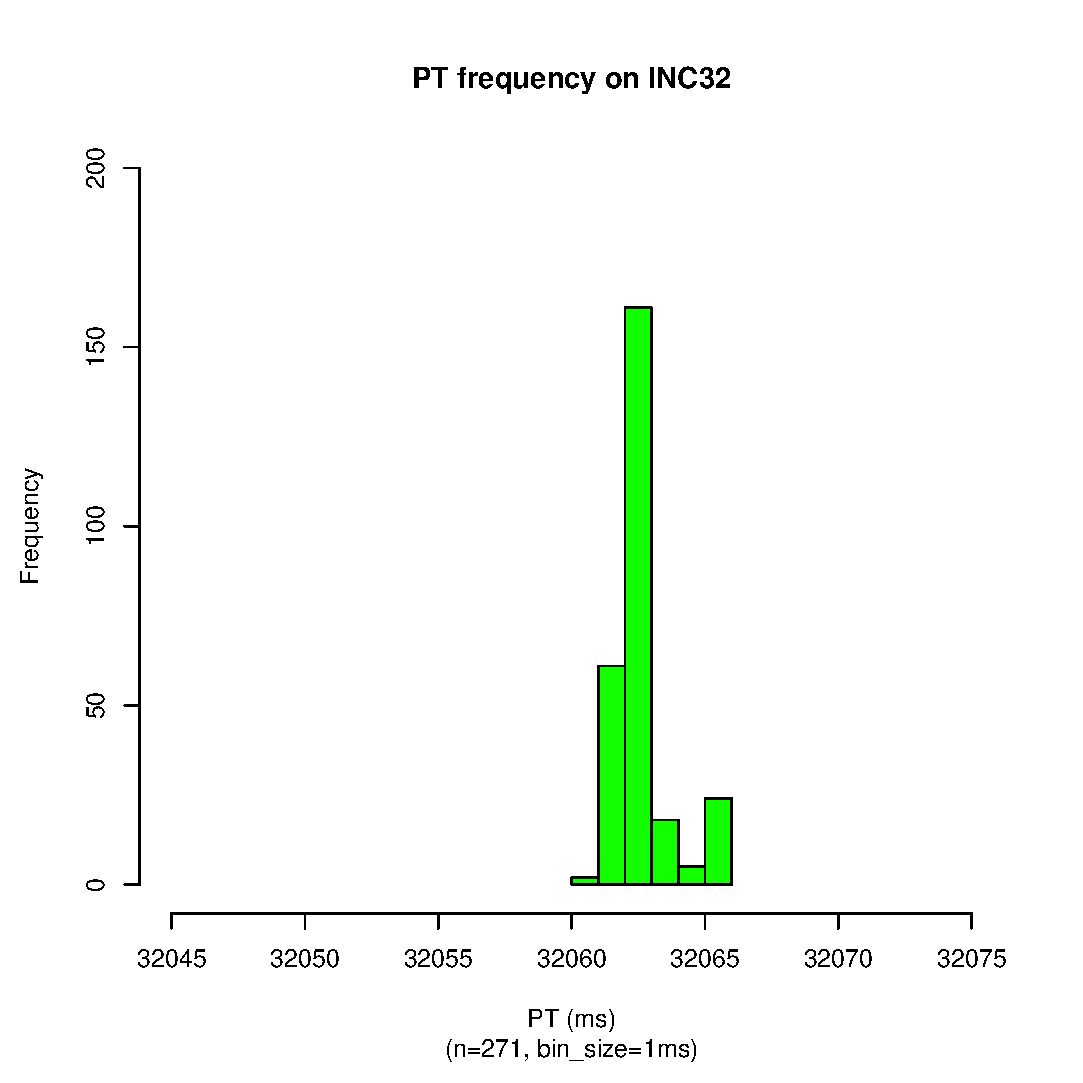
\includegraphics[scale=0.43]{sodb12/32_sec_pt_hist_v5.eps}
		\label{fig:s12_inc32_hist_v5}
	}
	\subfigure[PT frequency on INC64 on {\tt sodb12}]{
		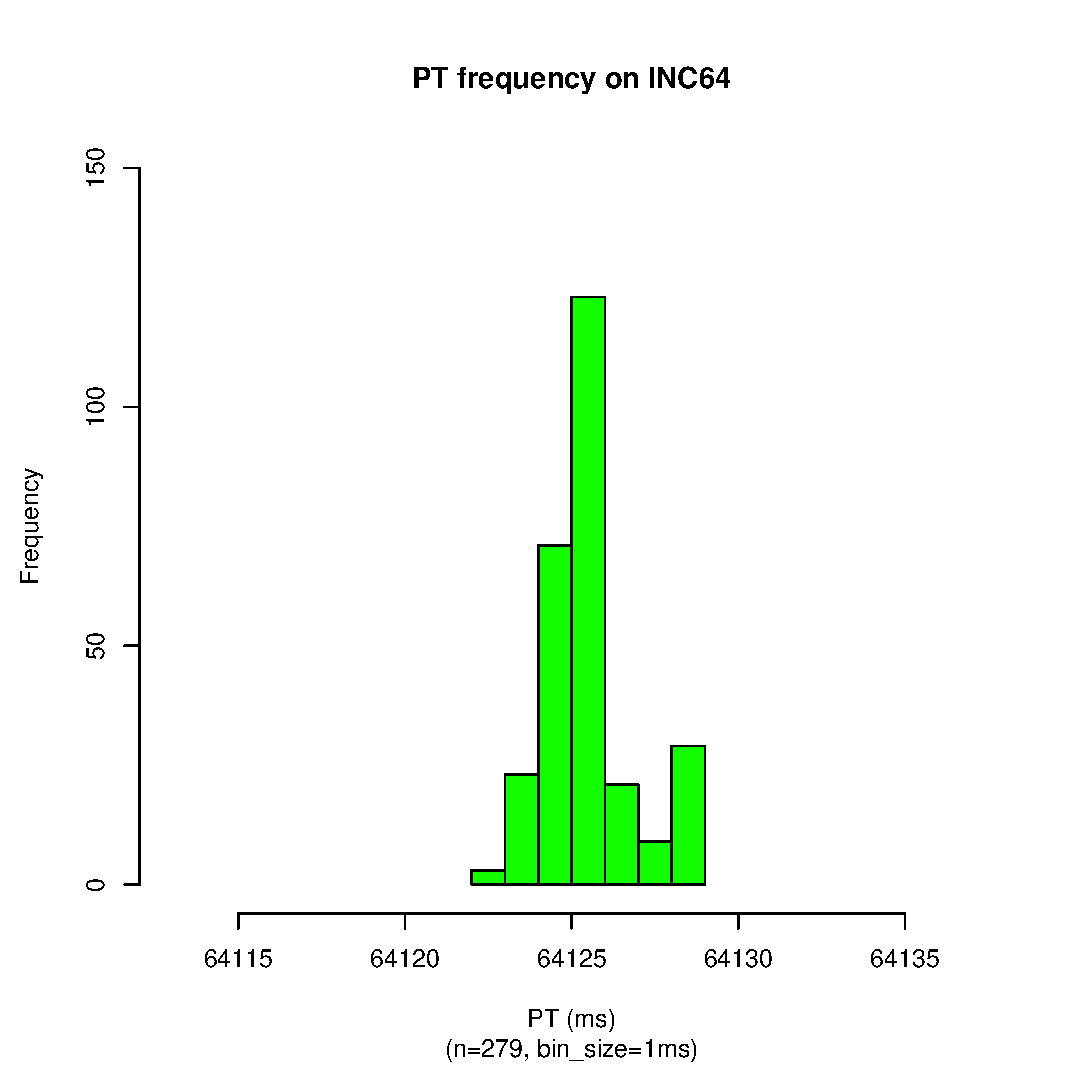
\includegraphics[scale=0.43]{sodb12/64_sec_pt_hist_v5.eps}
		\label{fig:s12_inc64_hist_v5}
	}
	\subfigure[PT frequency on INC128 on {\tt sodb12}]{
		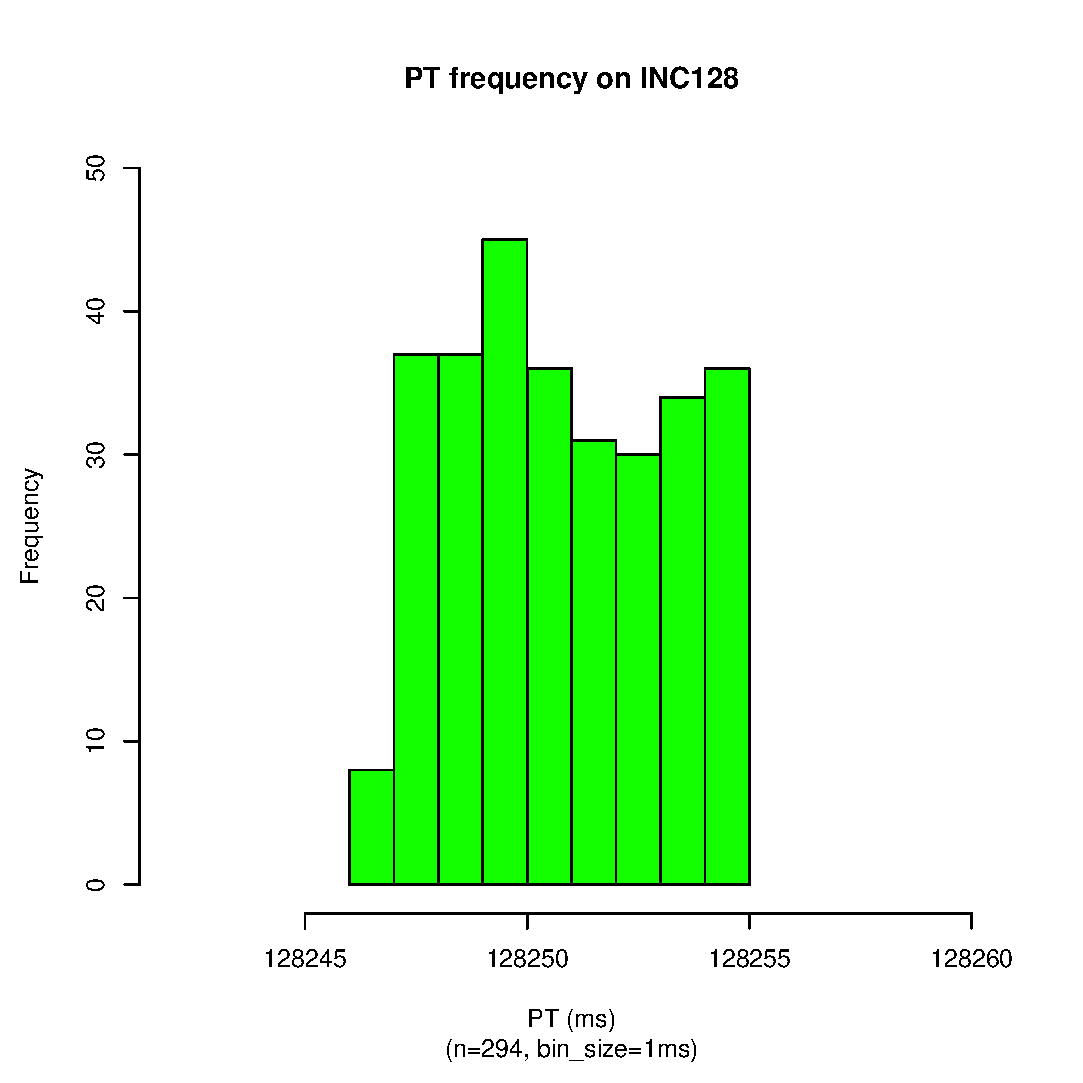
\includegraphics[scale=0.43]{sodb12/128_sec_pt_hist_v5.eps}
		\label{fig:s12_inc128_hist_v5}
	}
	\caption{PT Histograms of INC16 ... INC64~\label{fig:s12_pt_hist2}}
\end{figure}
\newpage

\subsection{{\tt sodb12}~\label{sec:sodb12_hist}} 
This section exhibits histograms on the EMPv5 data obtained on {\tt sodb12}. 
The detailed description of the base data are from Table~\ref{tab:exp_notes}.

\subsubsection{ET}

\begin{figure}[hp!]
	\centering
	\subfigure[ET frequency on INC1 on {\tt sodb12}]{
		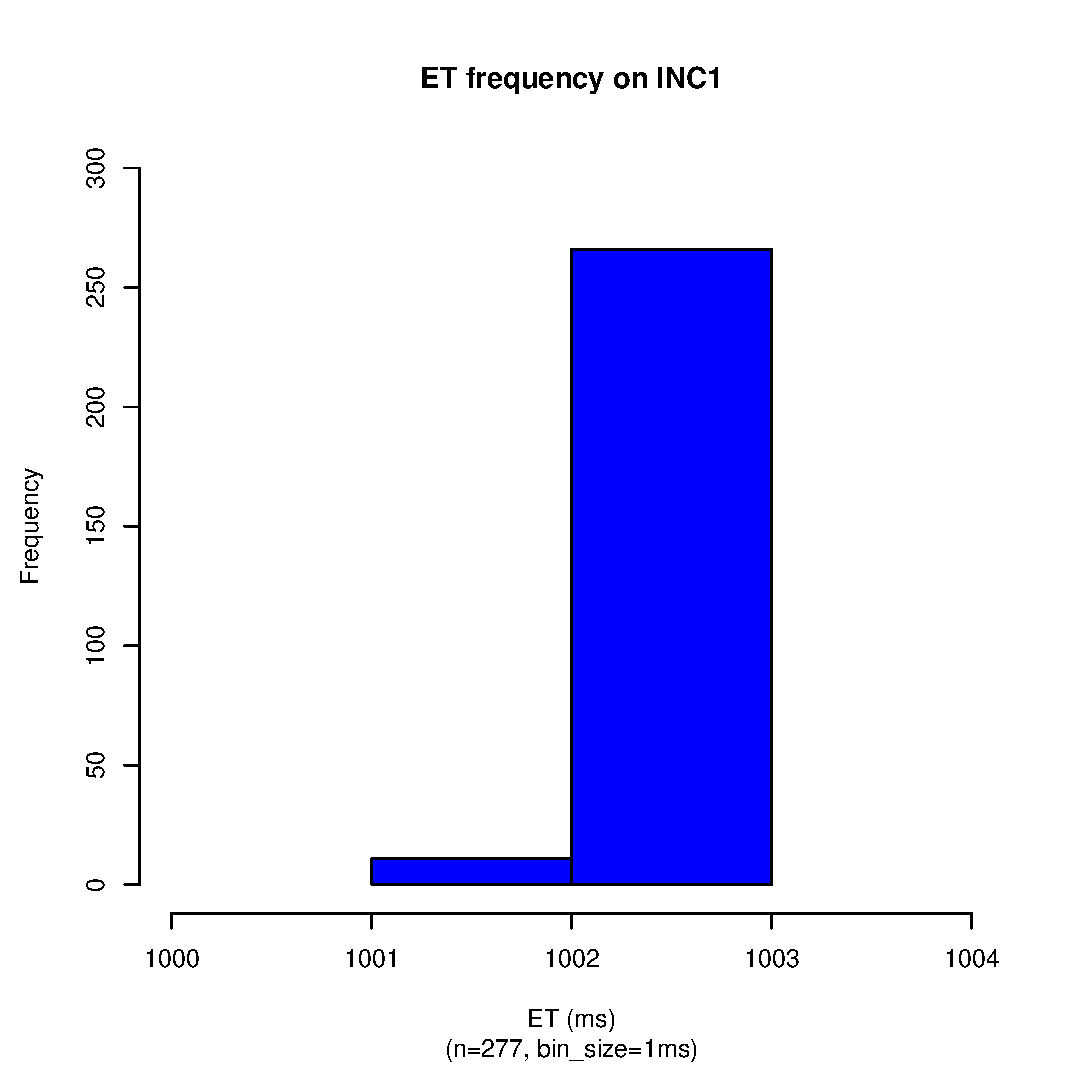
\includegraphics[scale=0.43]{sodb12/1_sec_et_hist_v5.eps}
		\label{fig:s12_inc1_et_hist_v5}
	}
	\subfigure[ET frequency on INC2 on {\tt sodb12}]{
		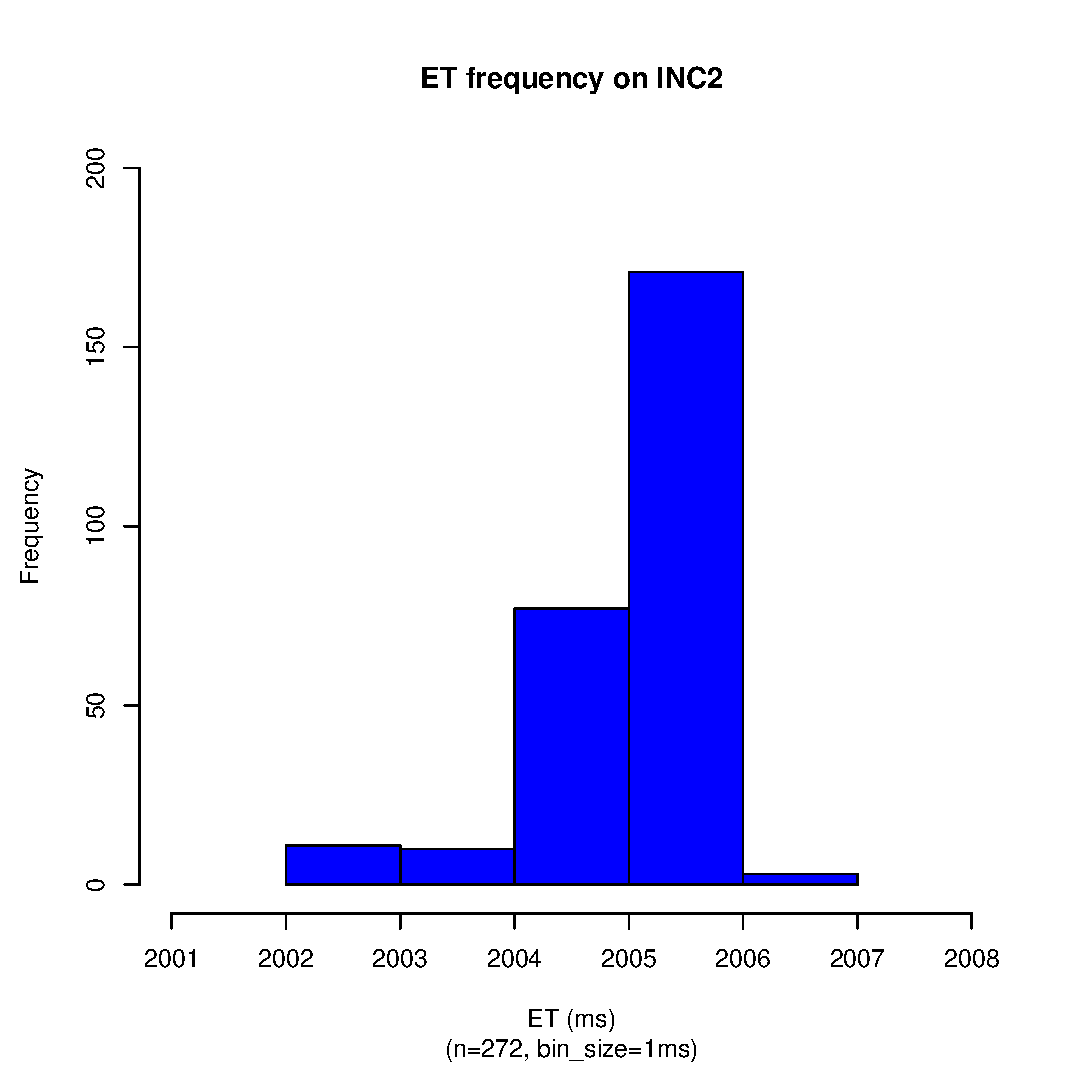
\includegraphics[scale=0.43]{sodb12/2_sec_et_hist_v5.eps}
		\label{fig:s12_inc2_et_hist_v5}
	}
	\subfigure[ET frequency on INC4 on {\tt sodb12}]{
		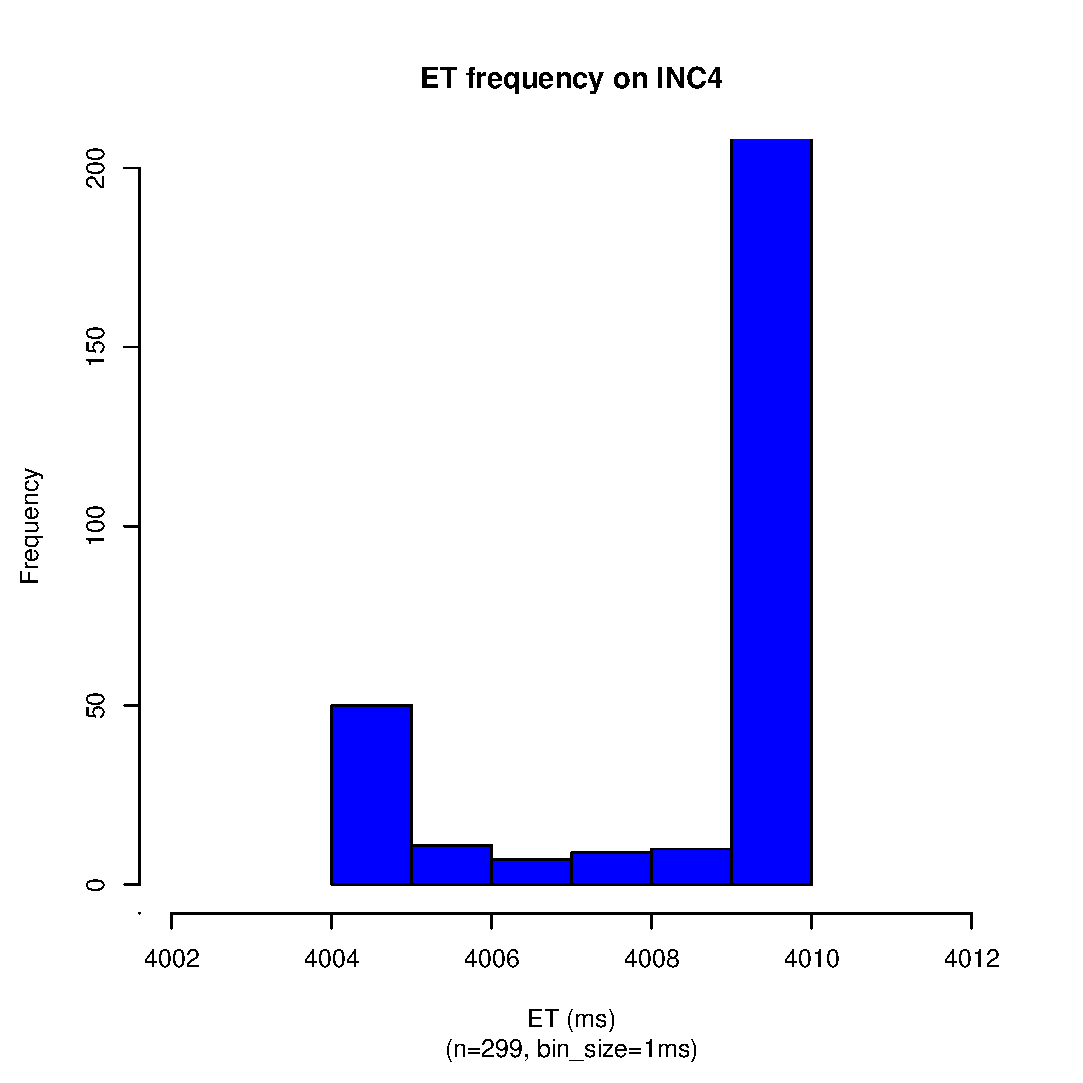
\includegraphics[scale=0.43]{sodb12/4_sec_et_hist_v5.eps}
		\label{fig:s12_inc4_et_hist_v5}
	}
	\subfigure[ET frequency on INC8 on {\tt sodb12}]{
		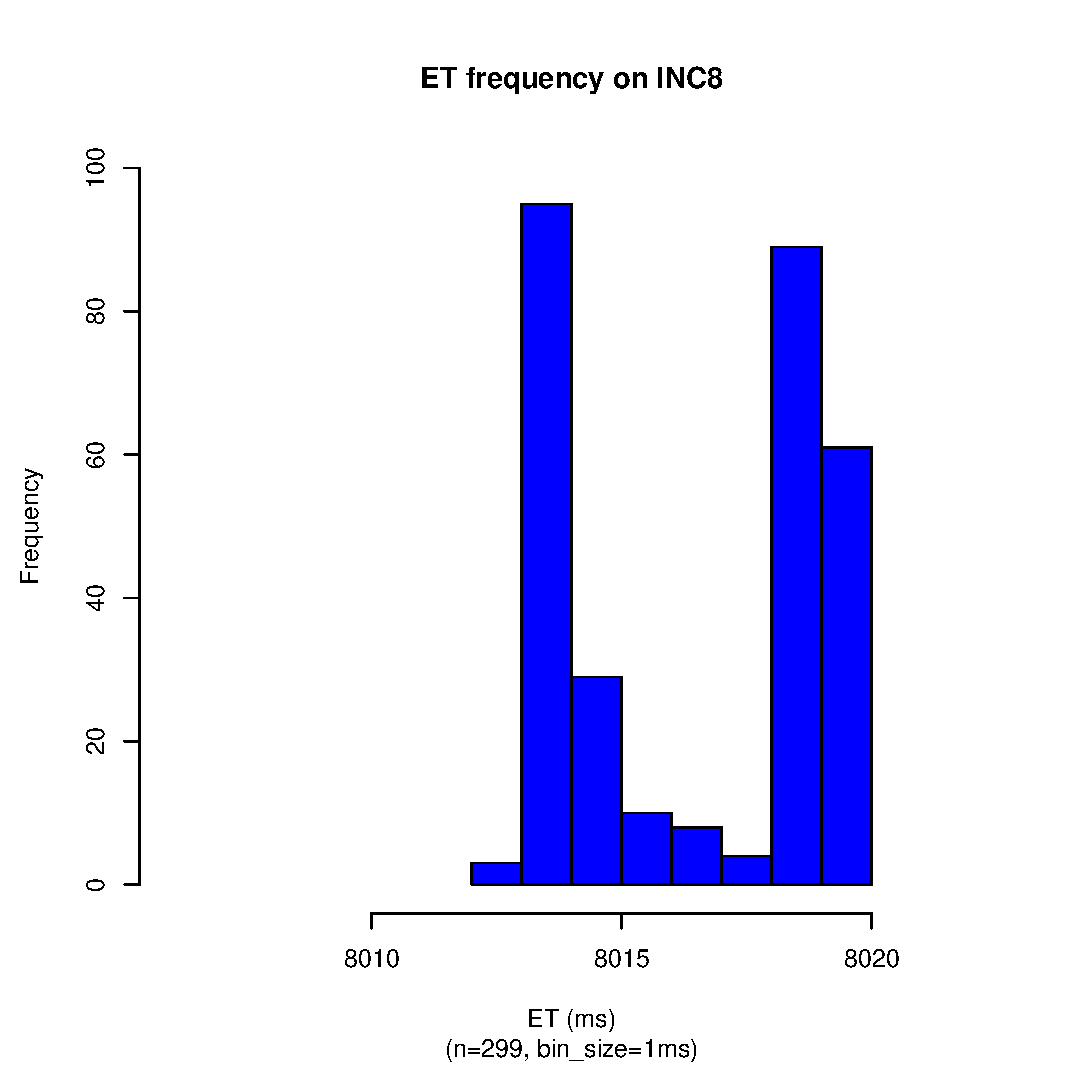
\includegraphics[scale=0.43]{sodb12/8_sec_et_hist_v5.eps}
		\label{fig:s12_inc8_et_hist_v5}
	}
	\caption{ET Histograms of INC1 ... INC8~\label{fig:s12_et_hist1}}
\end{figure}

\begin{figure}[hp!]
	\centering
	\subfigure[ET frequency on INC16 on {\tt sodb12}]{
		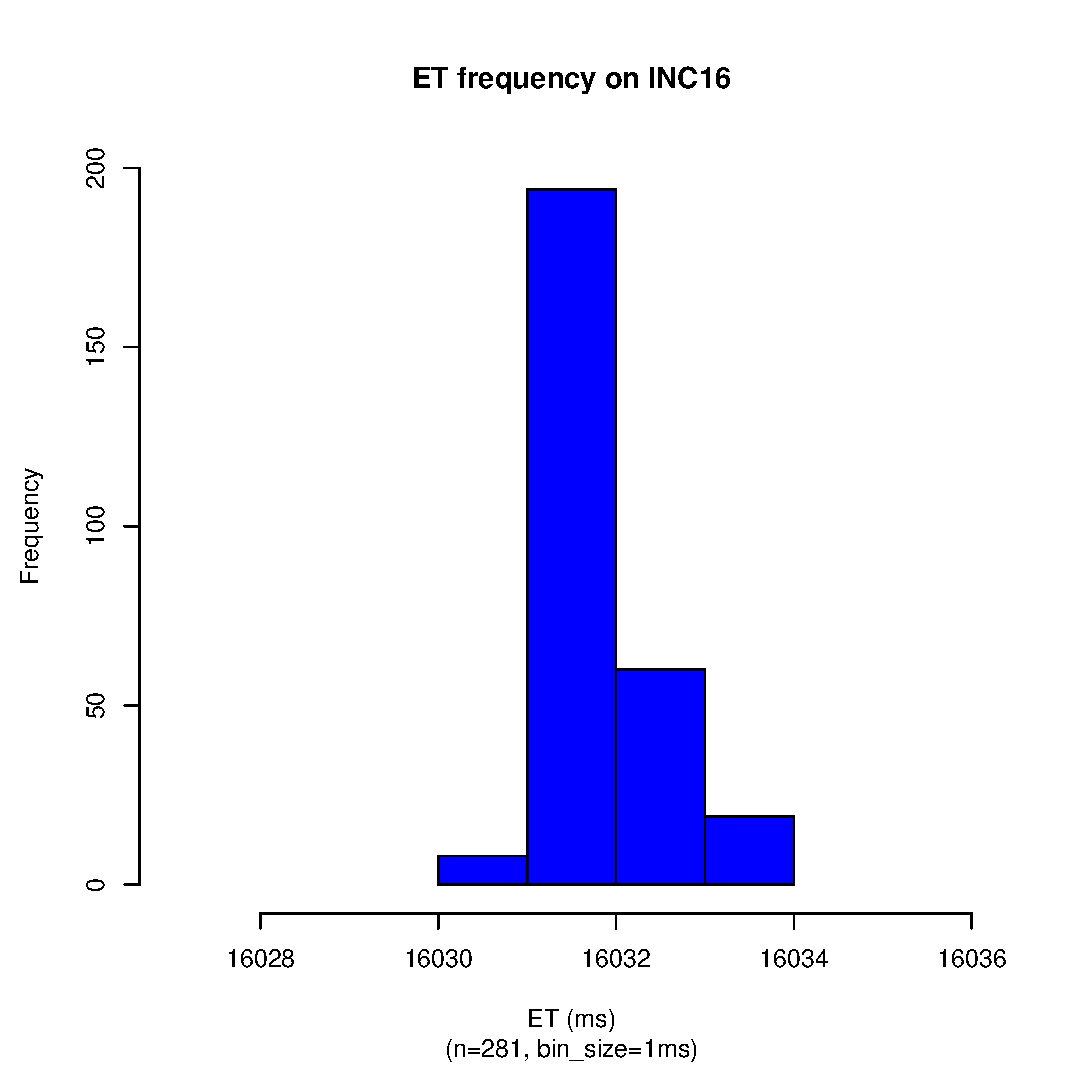
\includegraphics[scale=0.43]{sodb12/16_sec_et_hist_v5.eps}
		\label{fig:s12_inc16_et_hist_v5}
	}
	\subfigure[ET frequency on INC32 on {\tt sodb12}]{
		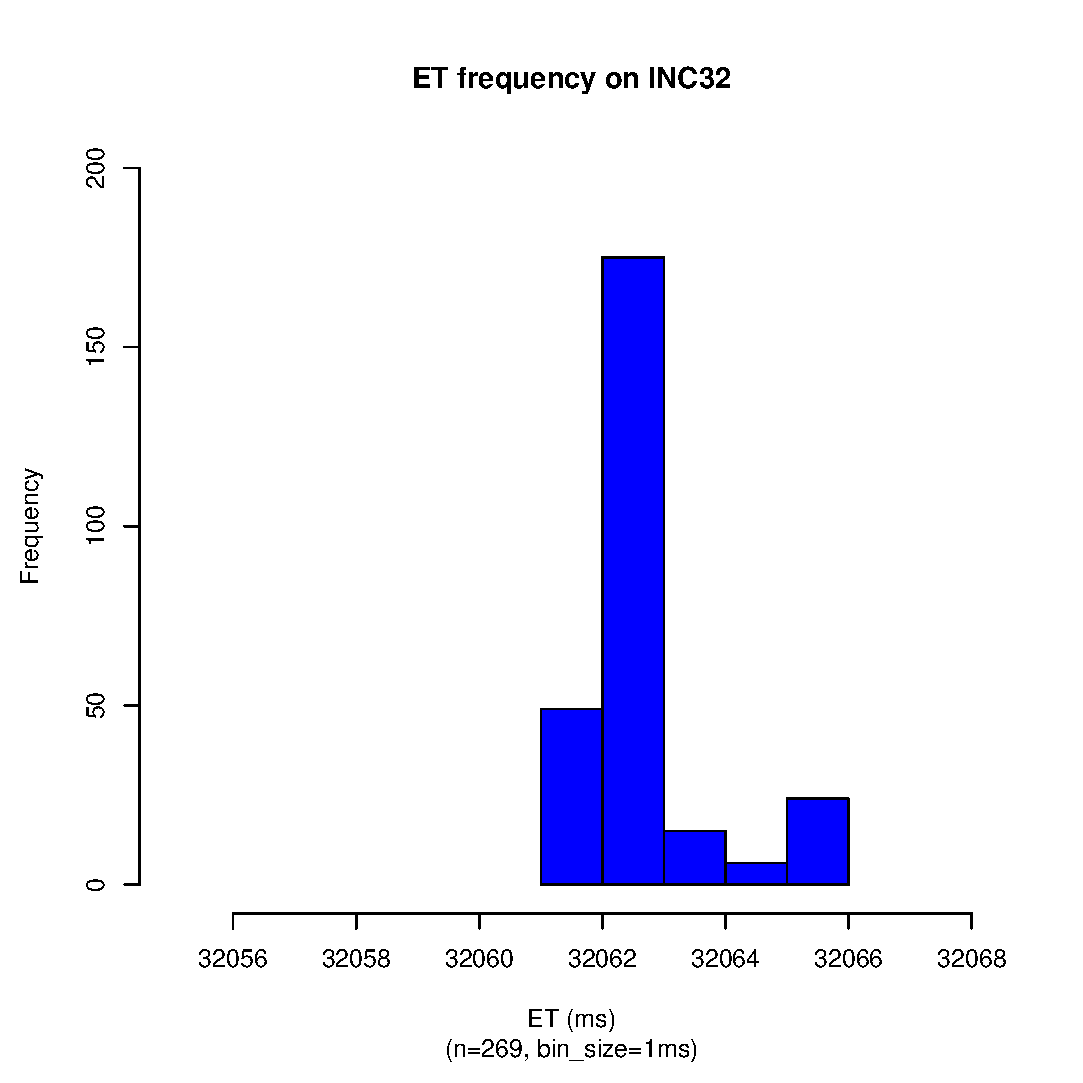
\includegraphics[scale=0.43]{sodb12/32_sec_et_hist_v5.eps}
		\label{fig:s12_inc32_et_hist_v5}
	}
	\subfigure[ET frequency on INC64 on {\tt sodb12}]{
		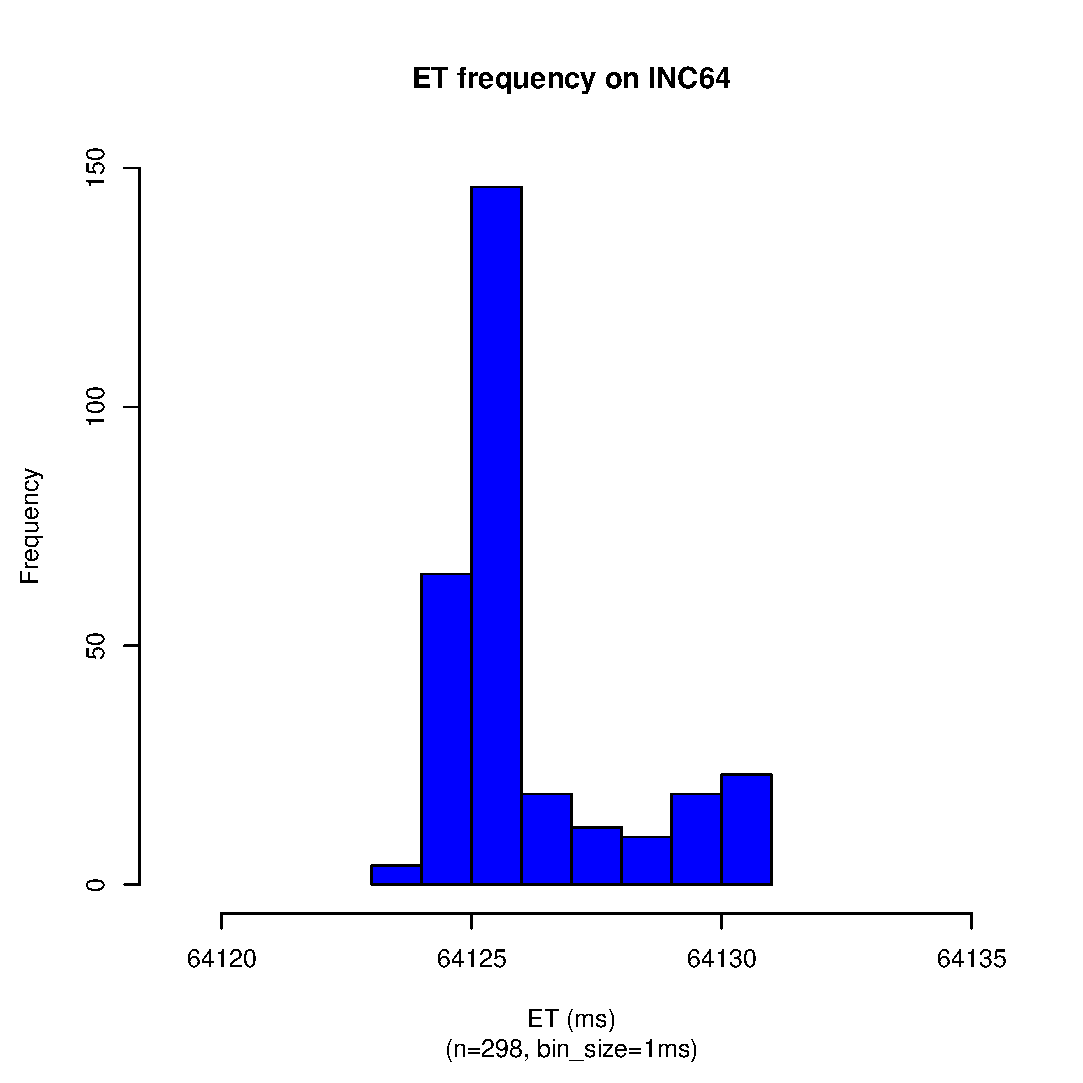
\includegraphics[scale=0.43]{sodb12/64_sec_et_hist_v5.eps}
		\label{fig:s12_inc64_et_hist_v5}
	}
	\subfigure[ET frequency on INC128 on {\tt sodb12}]{
		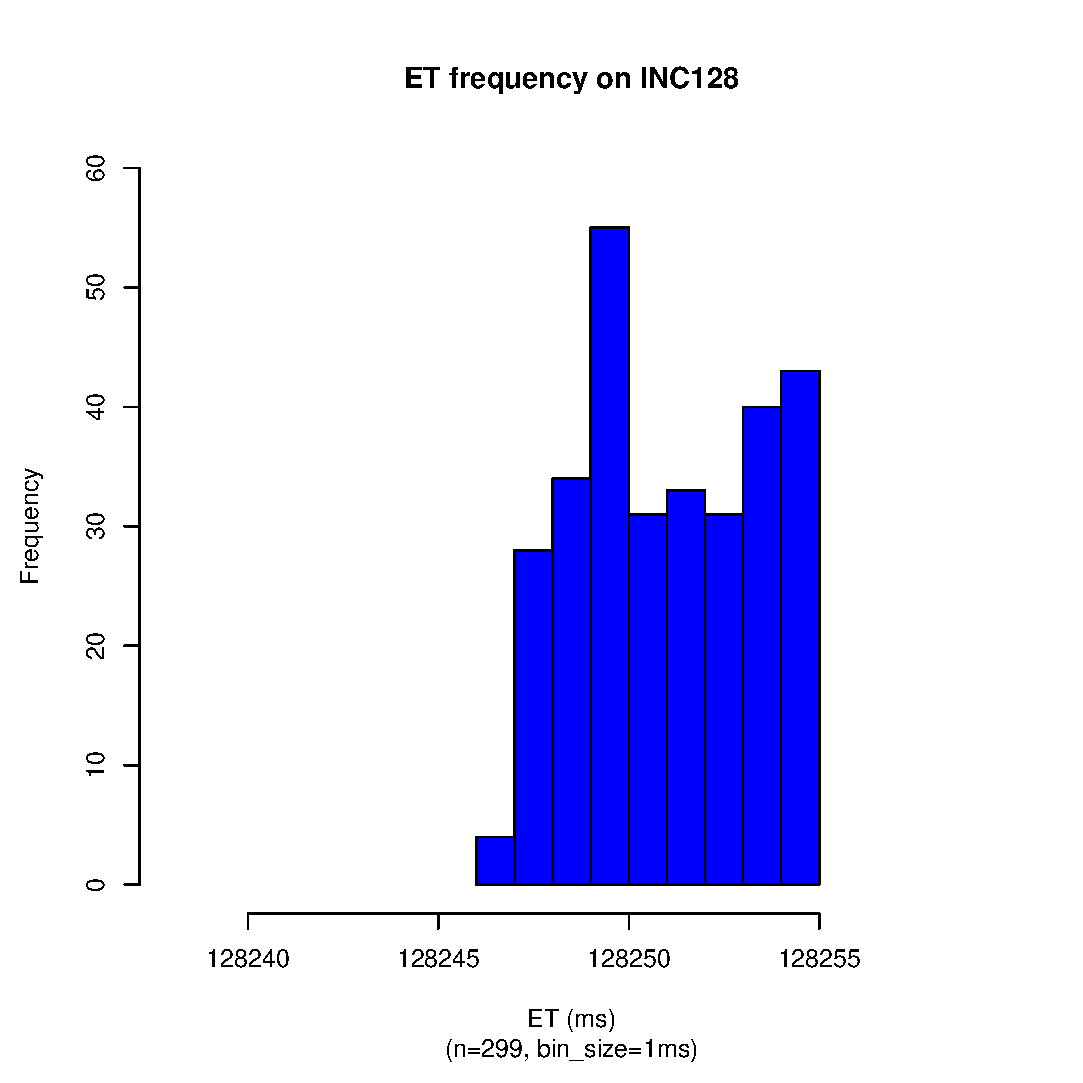
\includegraphics[scale=0.43]{sodb12/128_sec_et_hist_v5.eps}
		\label{fig:s12_inc128_et_hist_v5}
	}
	\caption{ET Histograms of INC16 ... INC128~\label{fig:s12_et_hist2}}
\end{figure}

\newpage

\subsubsection{PT}

\begin{figure}[hp!]
	\centering
	\subfigure[PT frequency on INC1 on {\tt sodb12}]{
		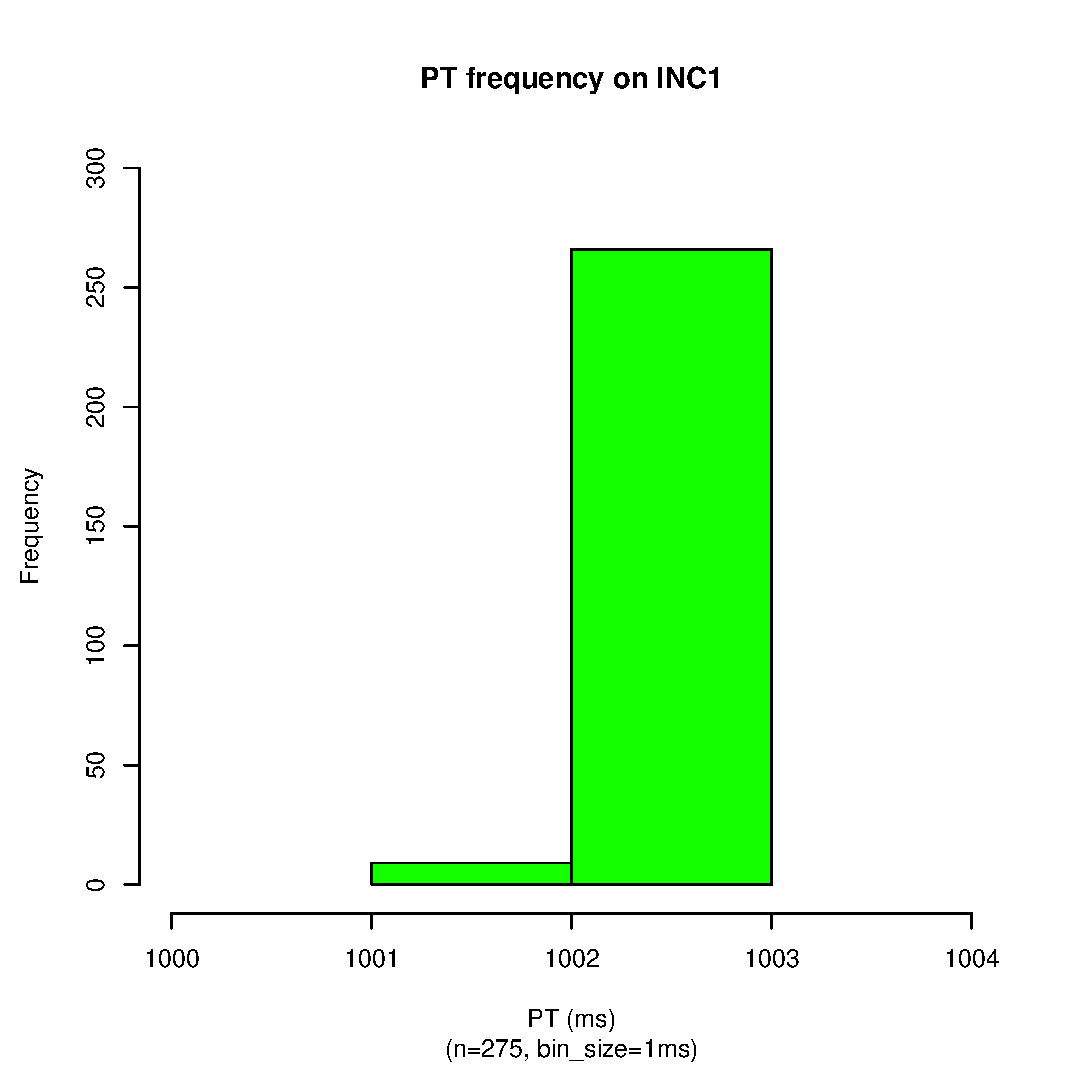
\includegraphics[scale=0.43]{sodb12/1_sec_pt_hist_v5.eps}
		\label{fig:s12_inc1_hist_v5}
	}
	\subfigure[PT frequency on INC2 on {\tt sodb12}]{
		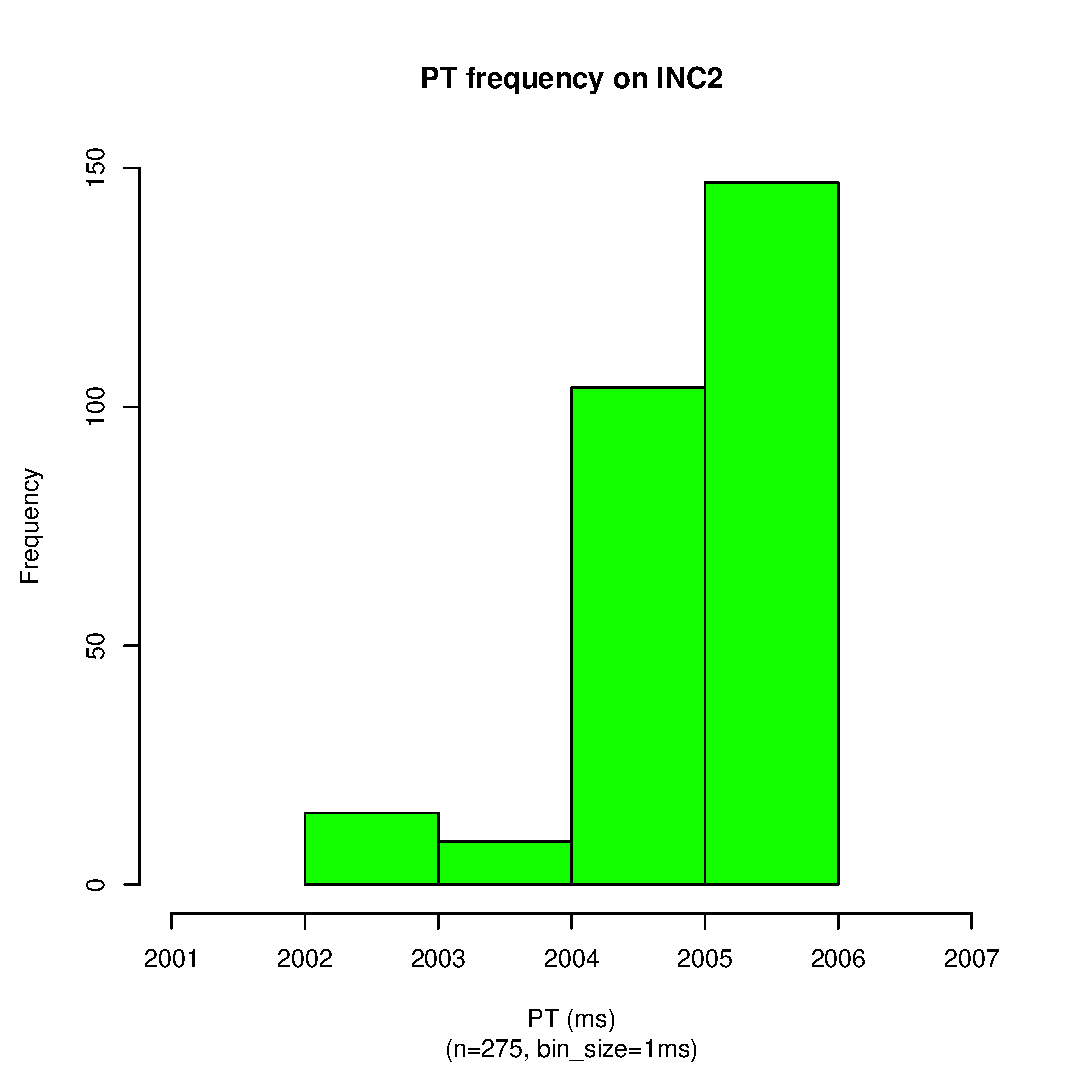
\includegraphics[scale=0.43]{sodb12/2_sec_pt_hist_v5.eps}
		\label{fig:s12_inc2_hist_v5}
	}
	\subfigure[PT frequency on INC4 on {\tt sodb12}]{
		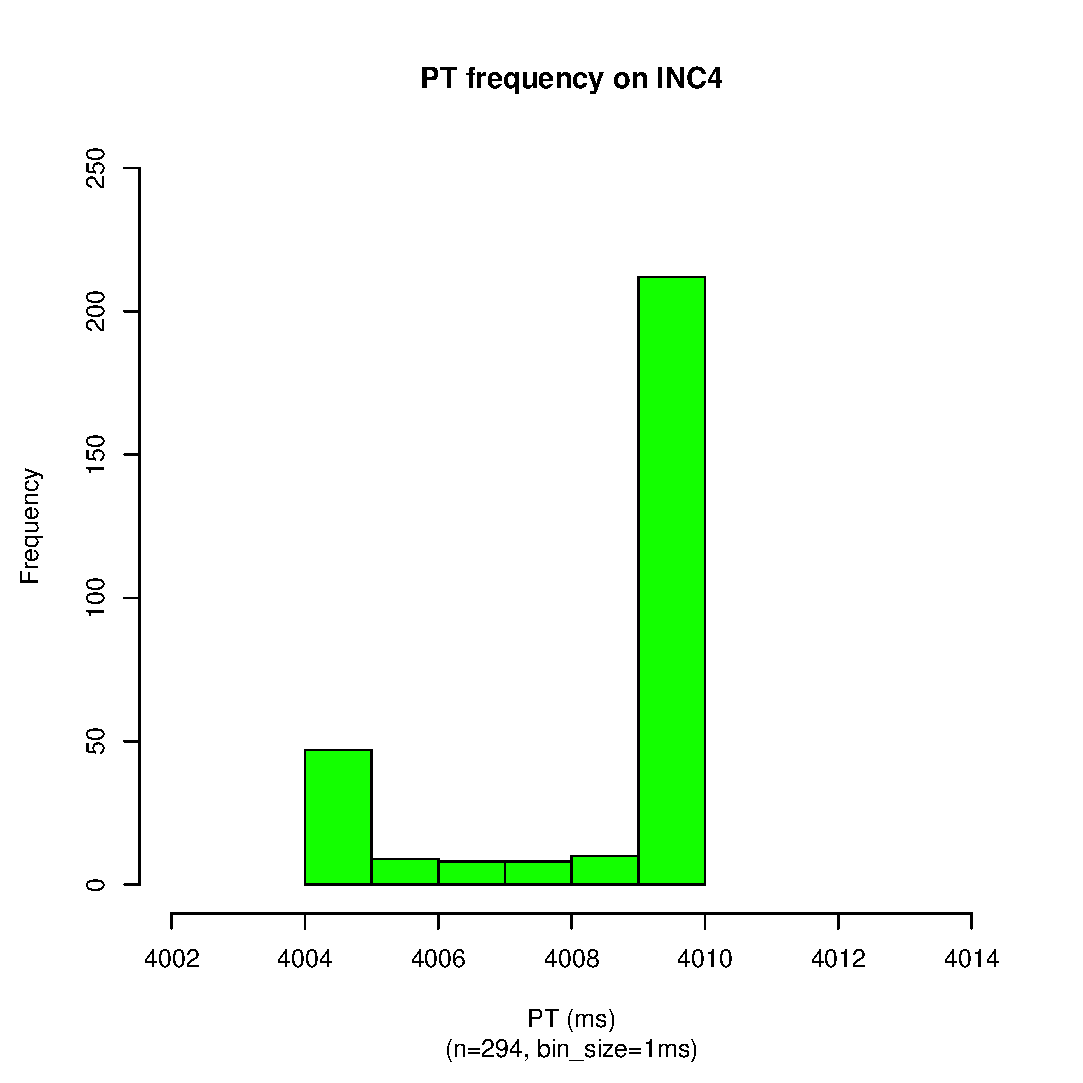
\includegraphics[scale=0.43]{sodb12/4_sec_pt_hist_v5.eps}
		\label{fig:s12_inc4_hist_v5}
	}
	\subfigure[PT frequency on INC8 on {\tt sodb12}]{
		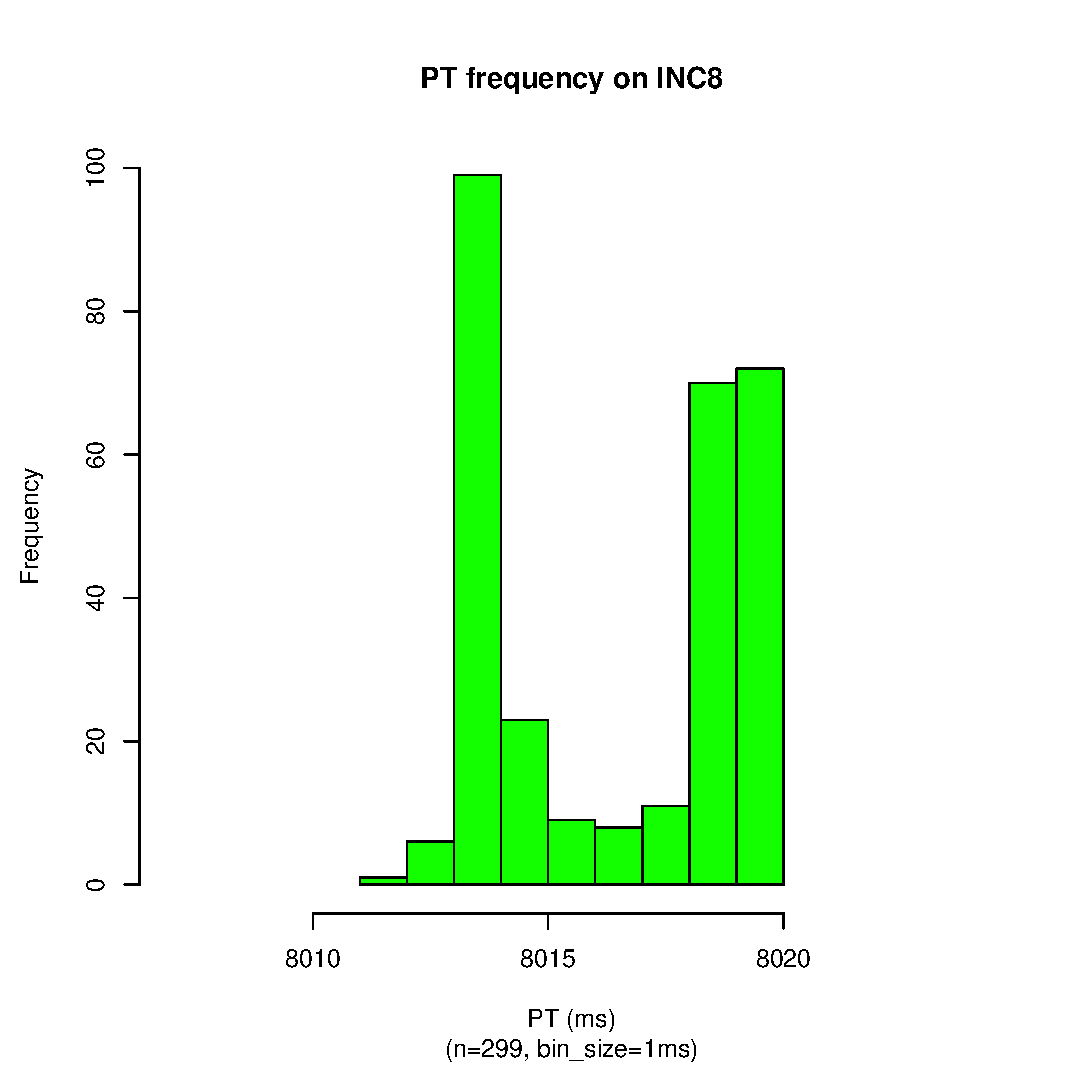
\includegraphics[scale=0.43]{sodb12/8_sec_pt_hist_v5.eps}
		\label{fig:s12_inc8_hist_v5}
	}
	\caption{PT Histograms of INC1 ... INC8~\label{fig:s12_pt_hist1}}
\end{figure}

\begin{figure}[hp!]
	\centering
	\subfigure[PT frequency on INC16 on {\tt sodb12}]{
		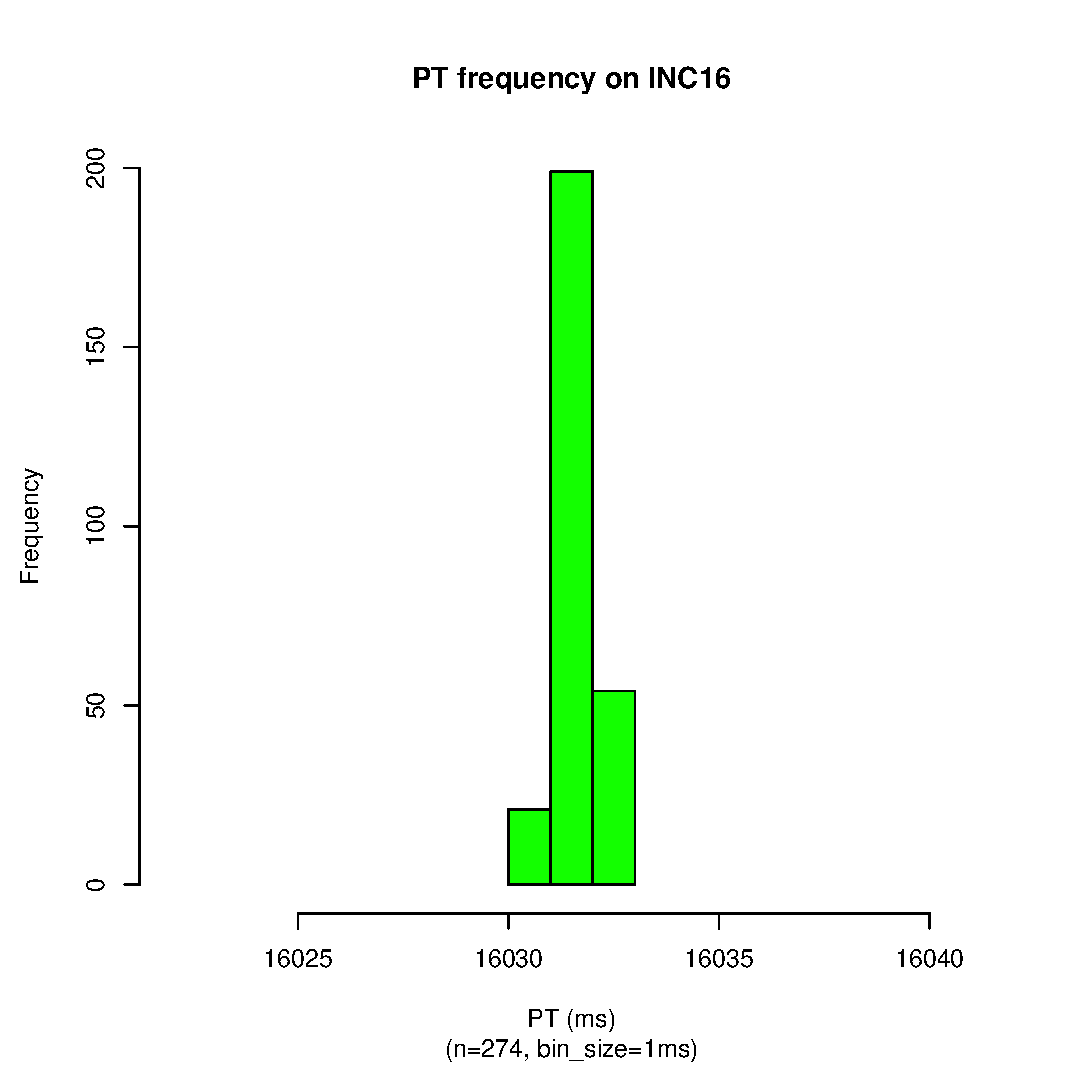
\includegraphics[scale=0.43]{sodb12/16_sec_pt_hist_v5.eps}
		\label{fig:s12_inc16_hist_v5}
	}
	\subfigure[PT frequency on INC32 on {\tt sodb12}]{
		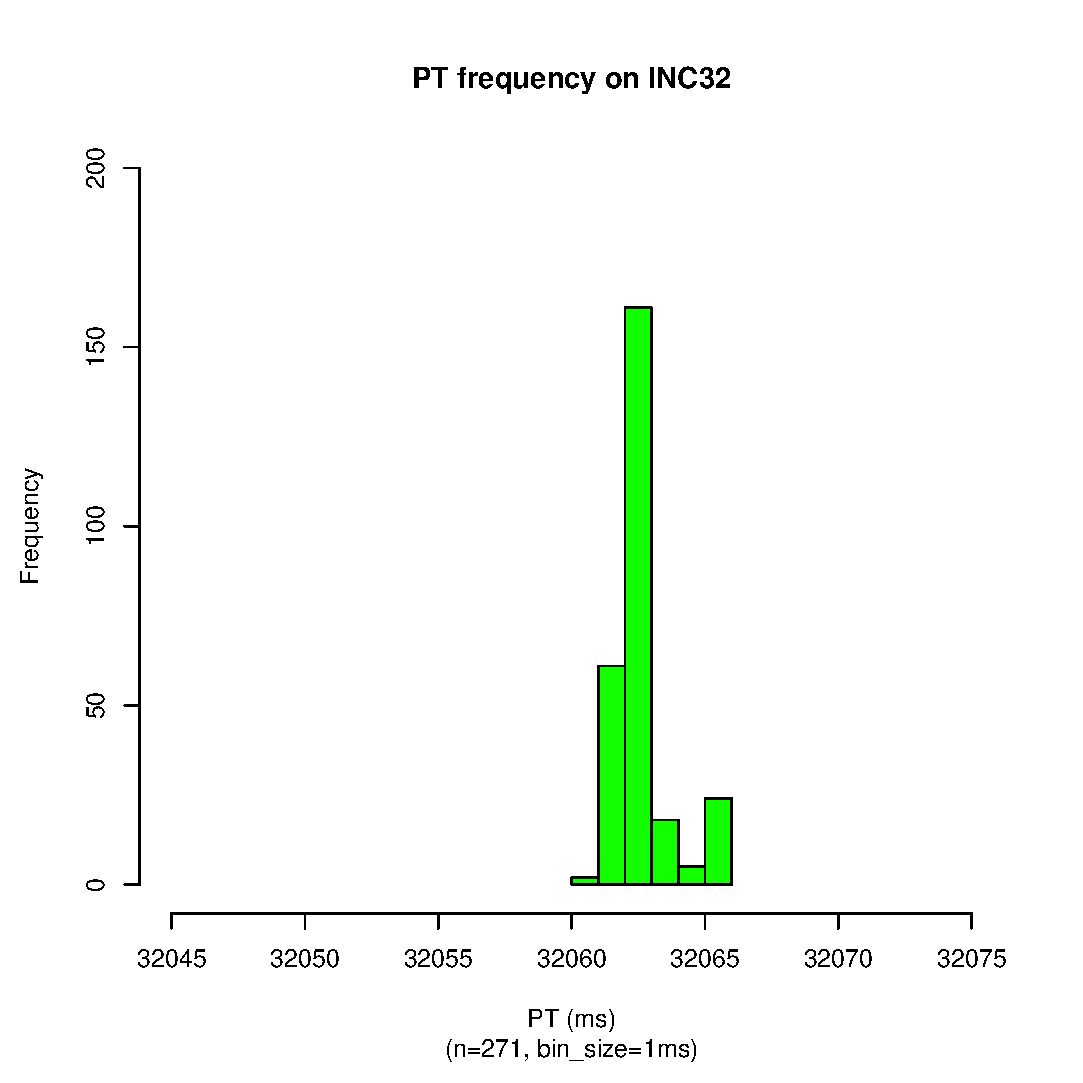
\includegraphics[scale=0.43]{sodb12/32_sec_pt_hist_v5.eps}
		\label{fig:s12_inc32_hist_v5}
	}
	\subfigure[PT frequency on INC64 on {\tt sodb12}]{
		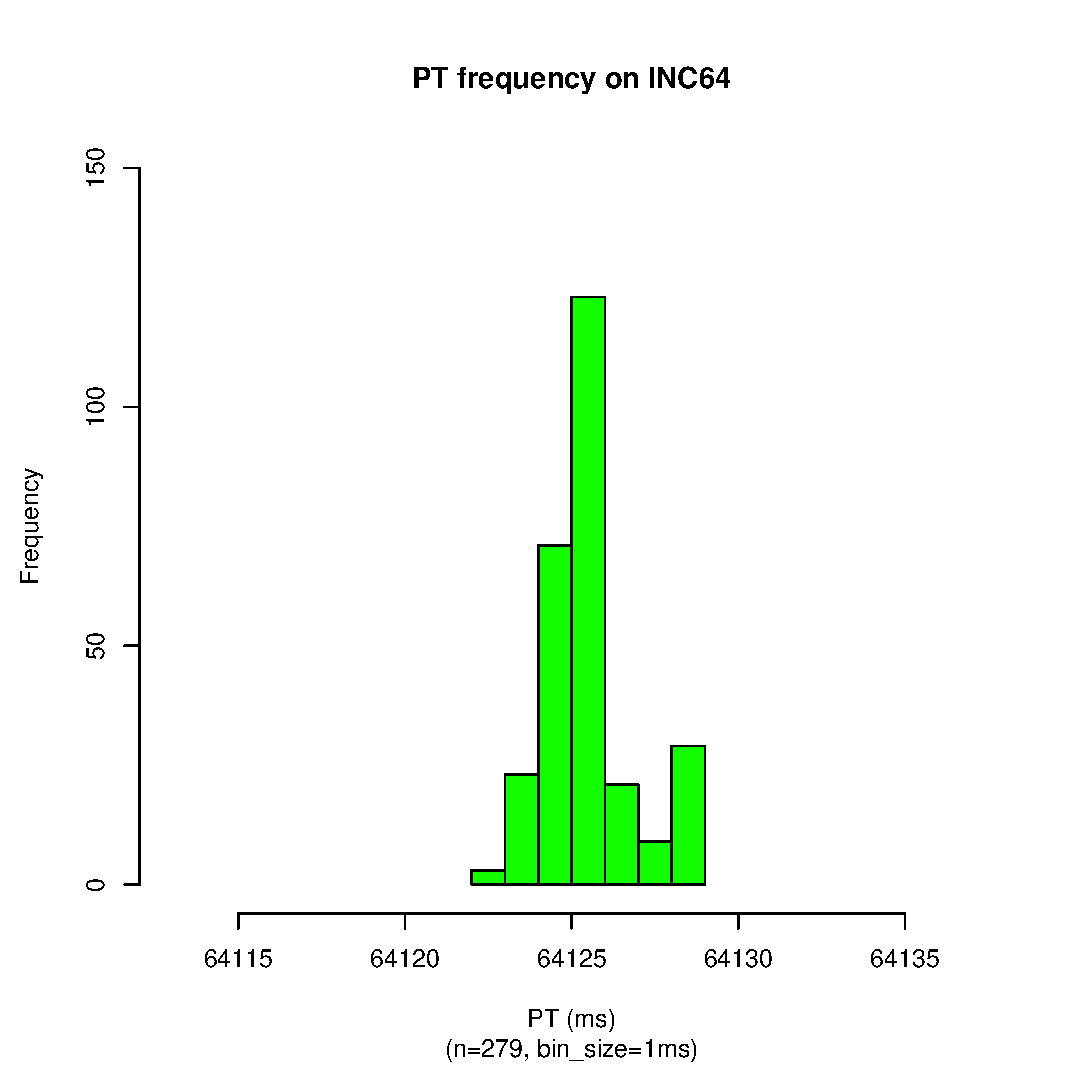
\includegraphics[scale=0.43]{sodb12/64_sec_pt_hist_v5.eps}
		\label{fig:s12_inc64_hist_v5}
	}
	\subfigure[PT frequency on INC128 on {\tt sodb12}]{
		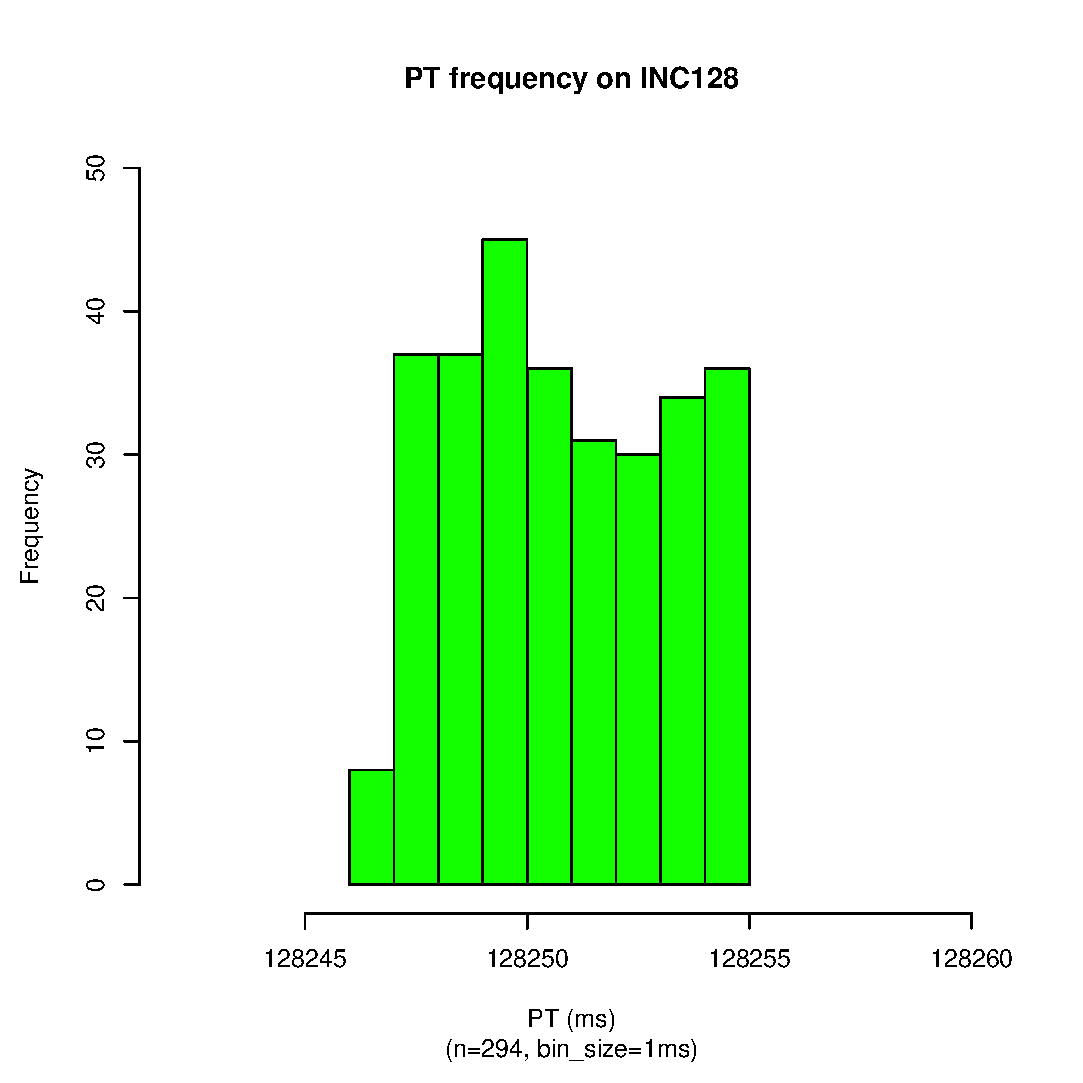
\includegraphics[scale=0.43]{sodb12/128_sec_pt_hist_v5.eps}
		\label{fig:s12_inc128_hist_v5}
	}
	\caption{PT Histograms of INC16 ... INC64~\label{fig:s12_pt_hist2}}
\end{figure}
\newpage

\subsection{{\tt sodb12}~\label{sec:sodb12_hist}} 
This section exhibits histograms on the EMPv5 data obtained on {\tt sodb12}. 
The detailed description of the base data are from Table~\ref{tab:exp_notes}.

\subsubsection{ET}

\begin{figure}[hp!]
	\centering
	\subfigure[ET frequency on INC1 on {\tt sodb12}]{
		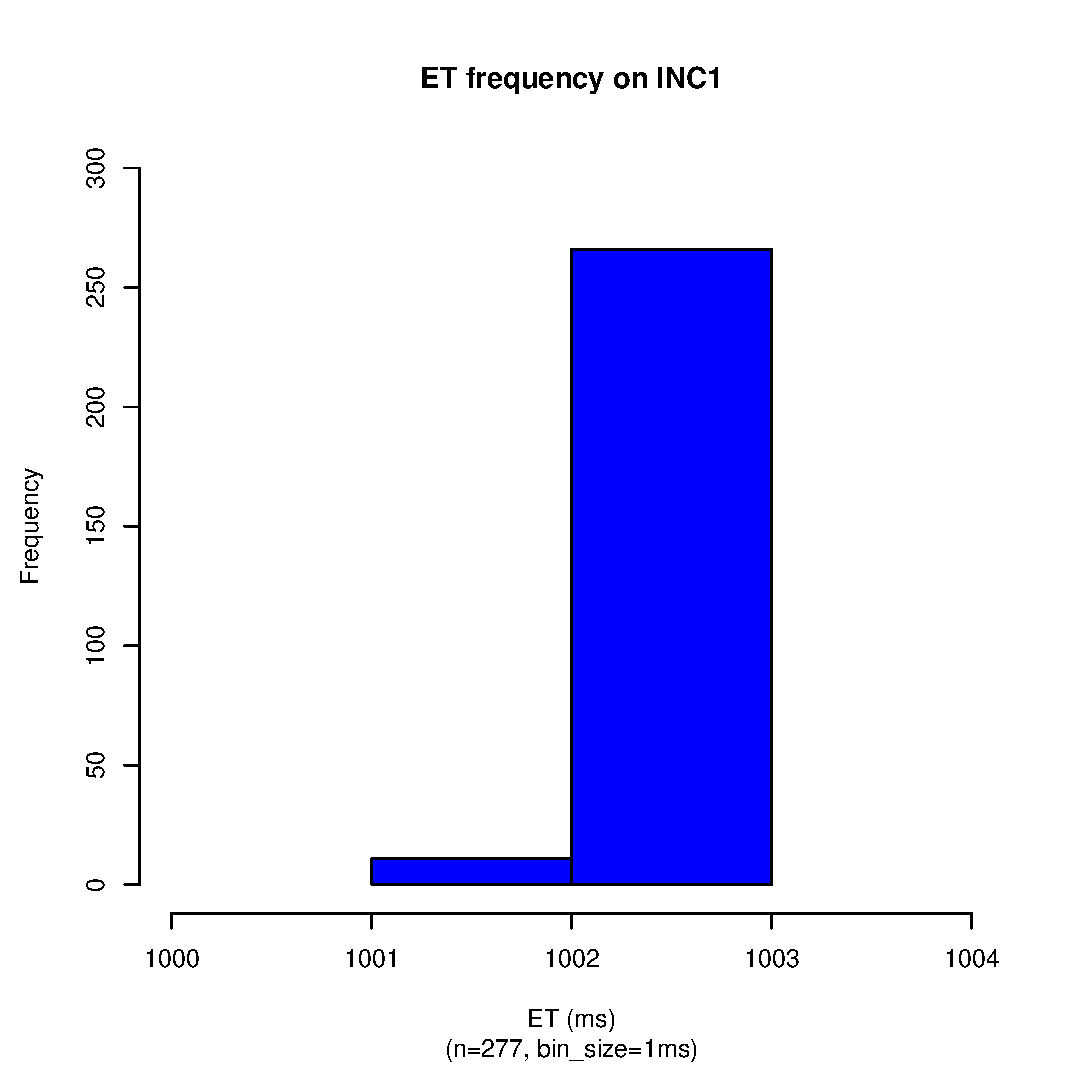
\includegraphics[scale=0.43]{sodb12/1_sec_et_hist_v5.eps}
		\label{fig:s12_inc1_et_hist_v5}
	}
	\subfigure[ET frequency on INC2 on {\tt sodb12}]{
		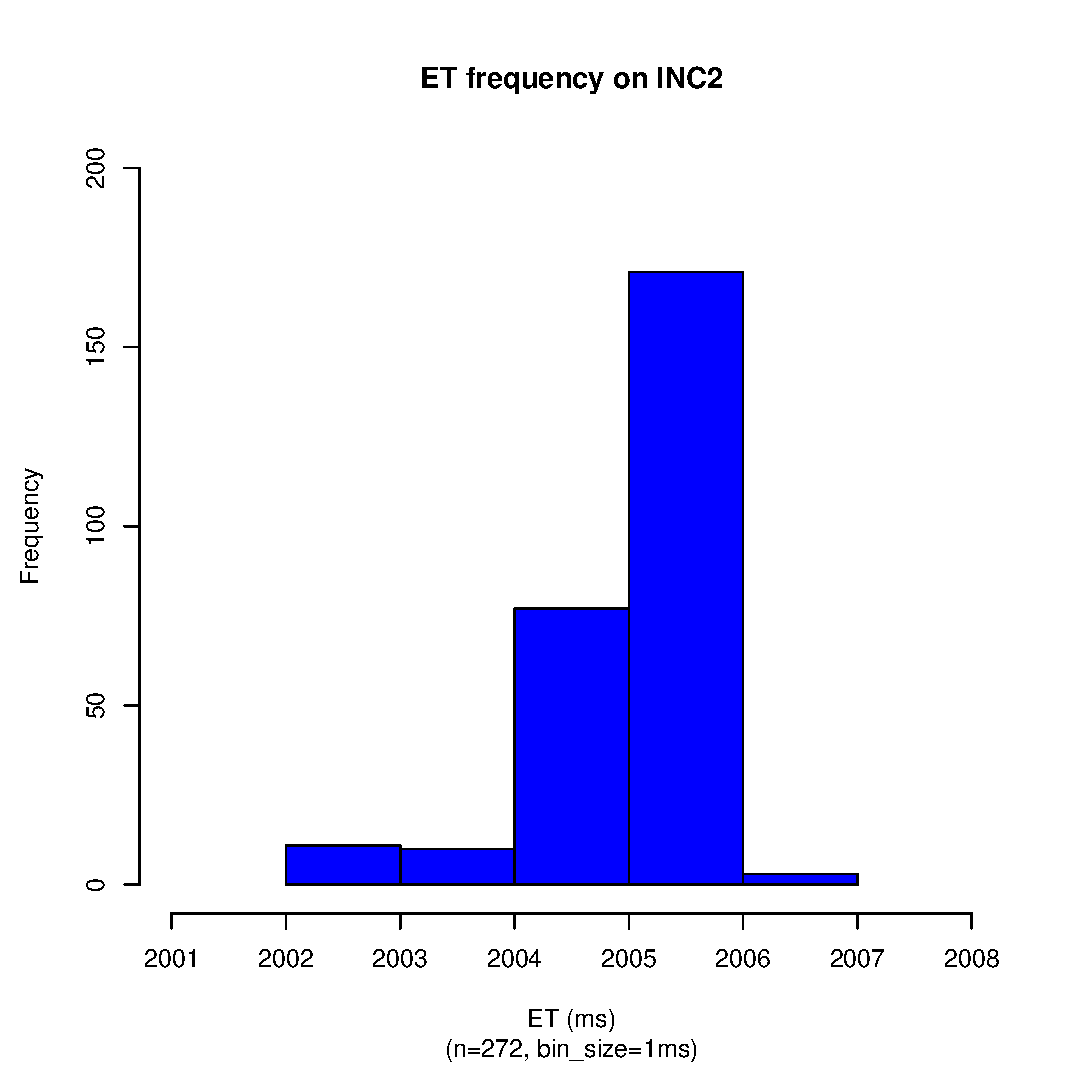
\includegraphics[scale=0.43]{sodb12/2_sec_et_hist_v5.eps}
		\label{fig:s12_inc2_et_hist_v5}
	}
	\subfigure[ET frequency on INC4 on {\tt sodb12}]{
		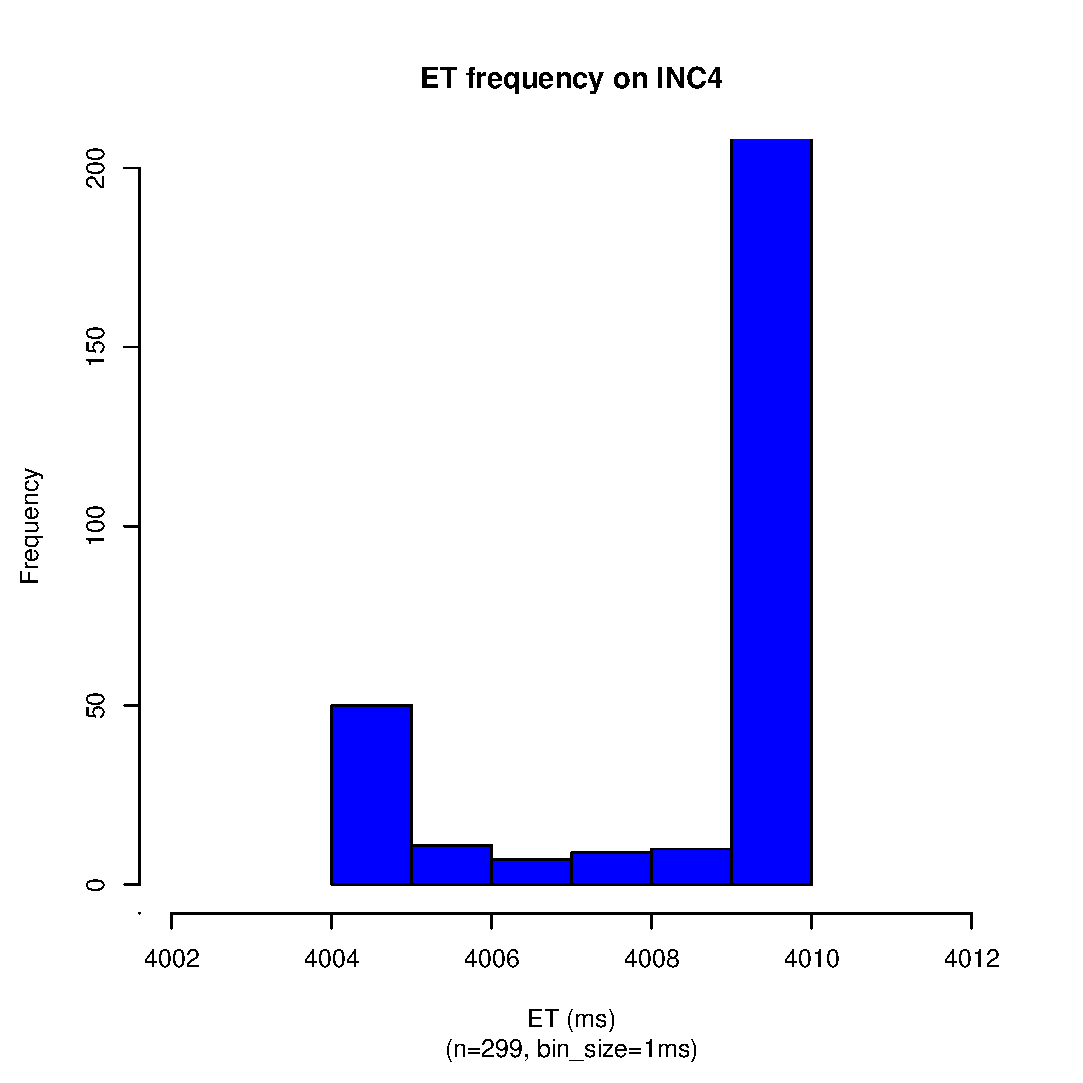
\includegraphics[scale=0.43]{sodb12/4_sec_et_hist_v5.eps}
		\label{fig:s12_inc4_et_hist_v5}
	}
	\subfigure[ET frequency on INC8 on {\tt sodb12}]{
		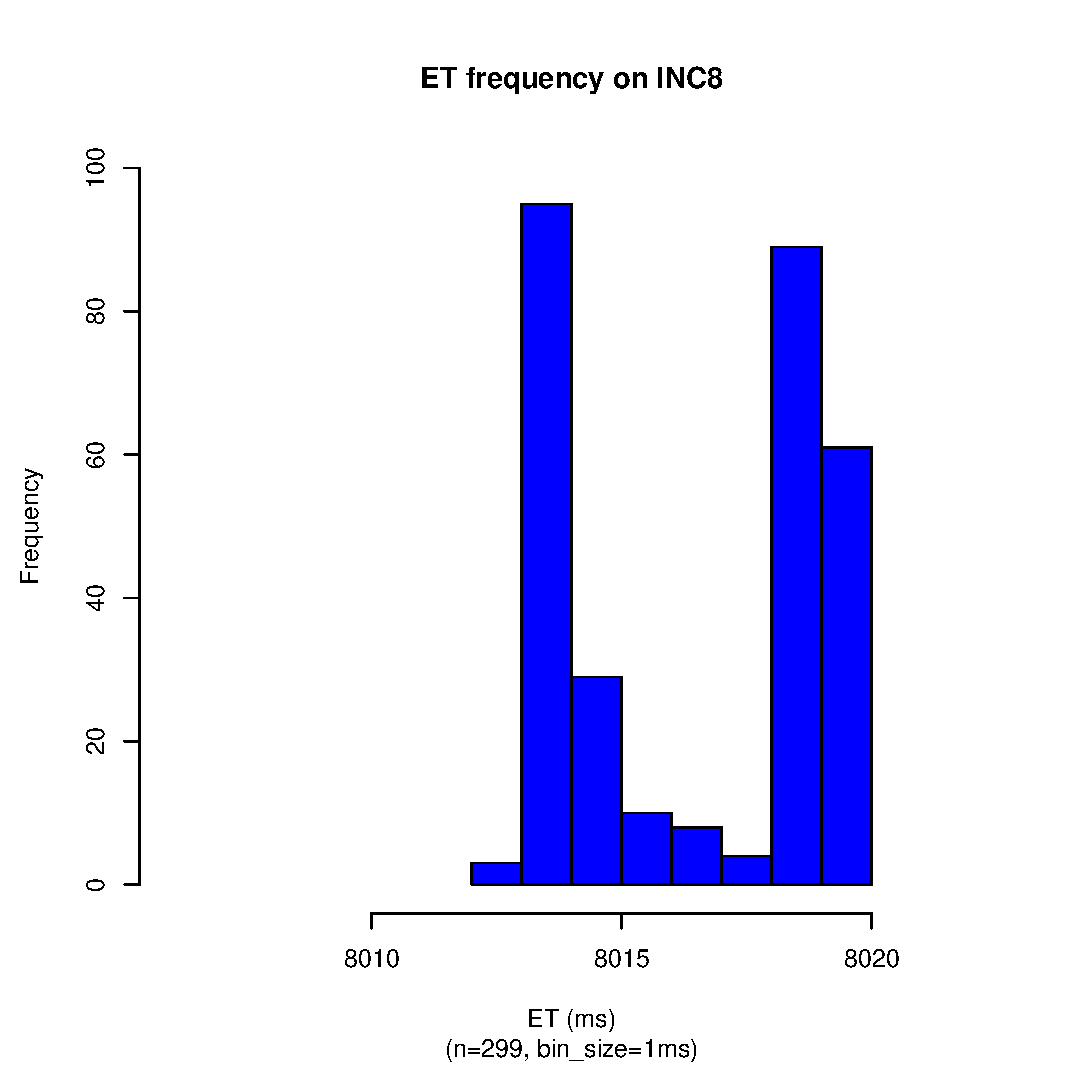
\includegraphics[scale=0.43]{sodb12/8_sec_et_hist_v5.eps}
		\label{fig:s12_inc8_et_hist_v5}
	}
	\caption{ET Histograms of INC1 ... INC8~\label{fig:s12_et_hist1}}
\end{figure}

\begin{figure}[hp!]
	\centering
	\subfigure[ET frequency on INC16 on {\tt sodb12}]{
		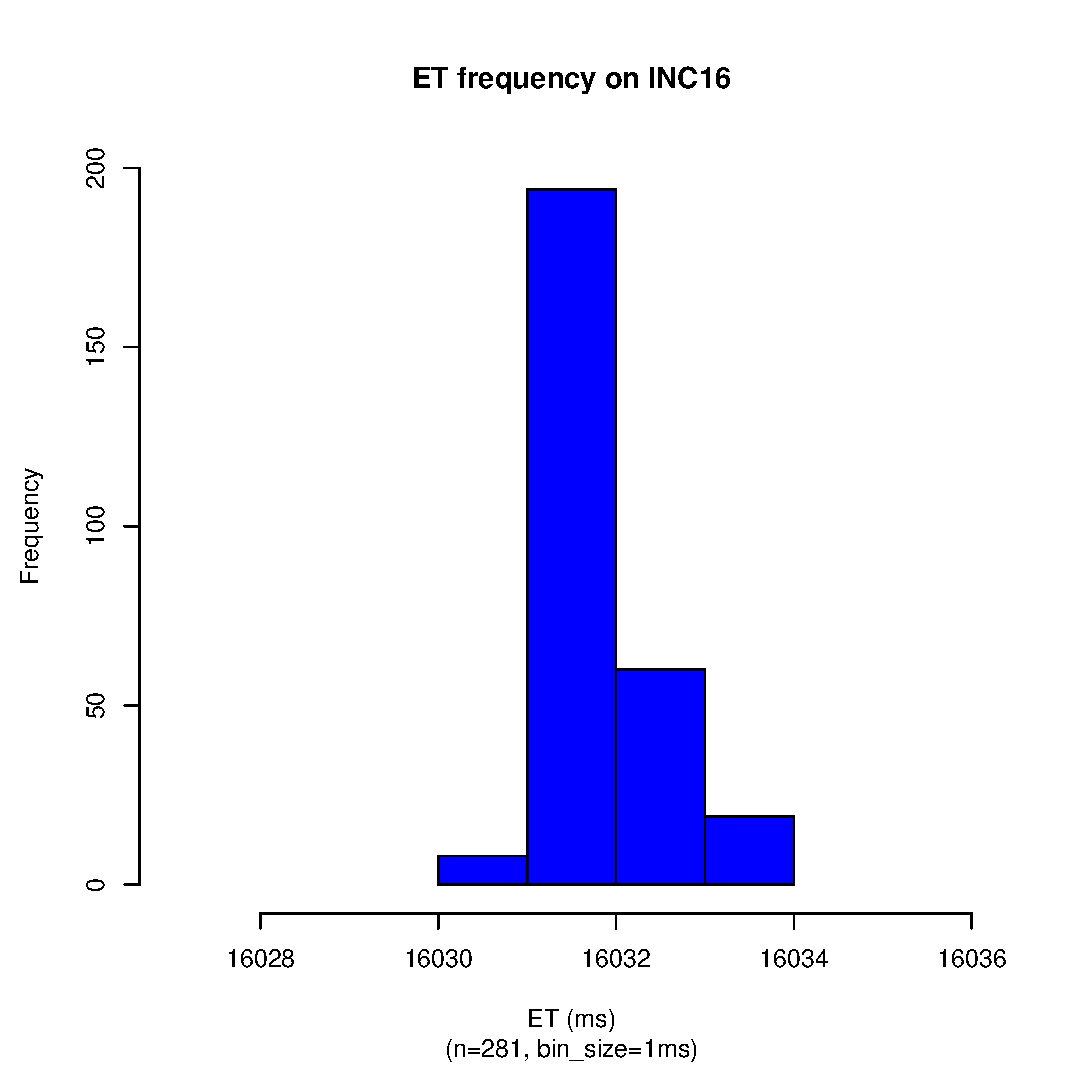
\includegraphics[scale=0.43]{sodb12/16_sec_et_hist_v5.eps}
		\label{fig:s12_inc16_et_hist_v5}
	}
	\subfigure[ET frequency on INC32 on {\tt sodb12}]{
		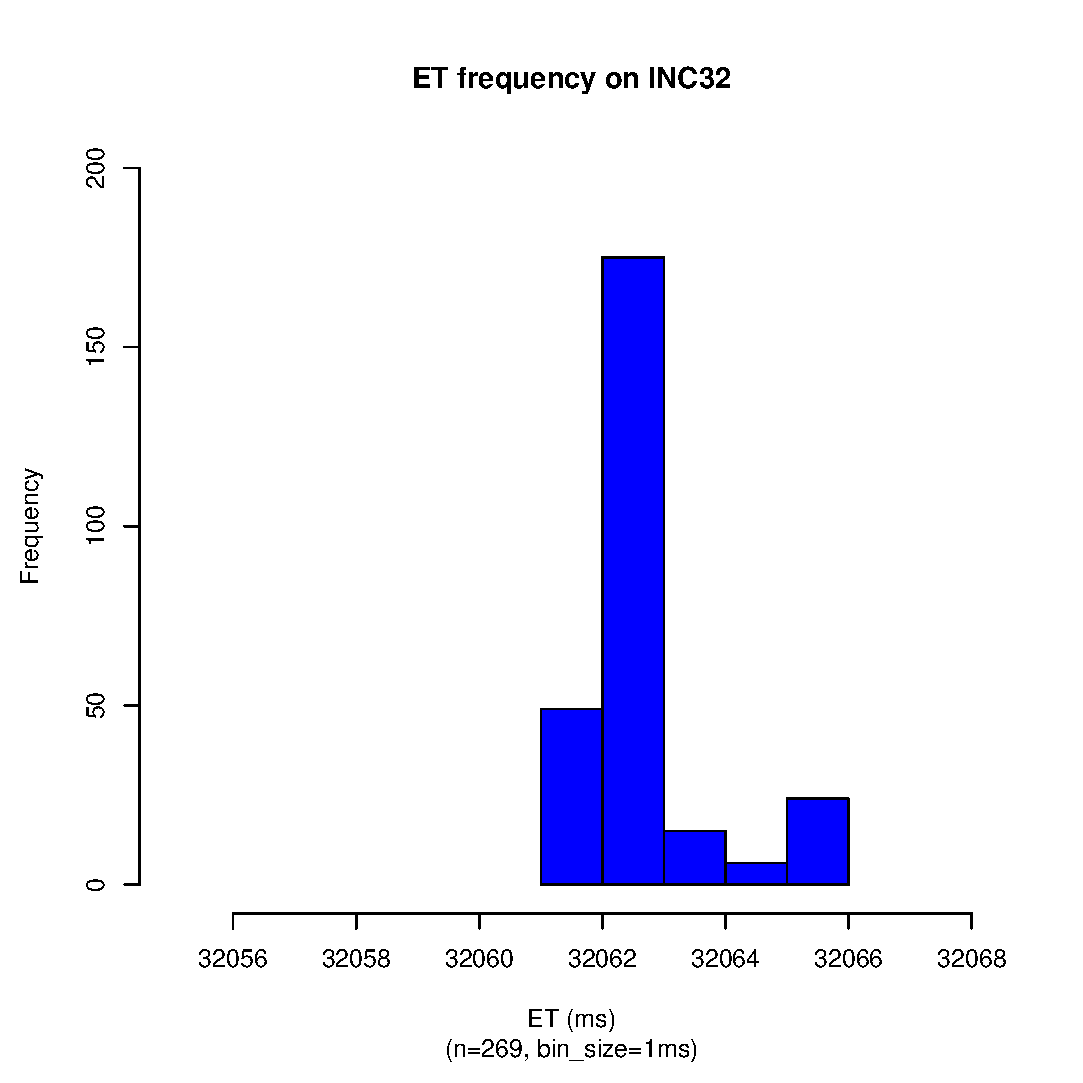
\includegraphics[scale=0.43]{sodb12/32_sec_et_hist_v5.eps}
		\label{fig:s12_inc32_et_hist_v5}
	}
	\subfigure[ET frequency on INC64 on {\tt sodb12}]{
		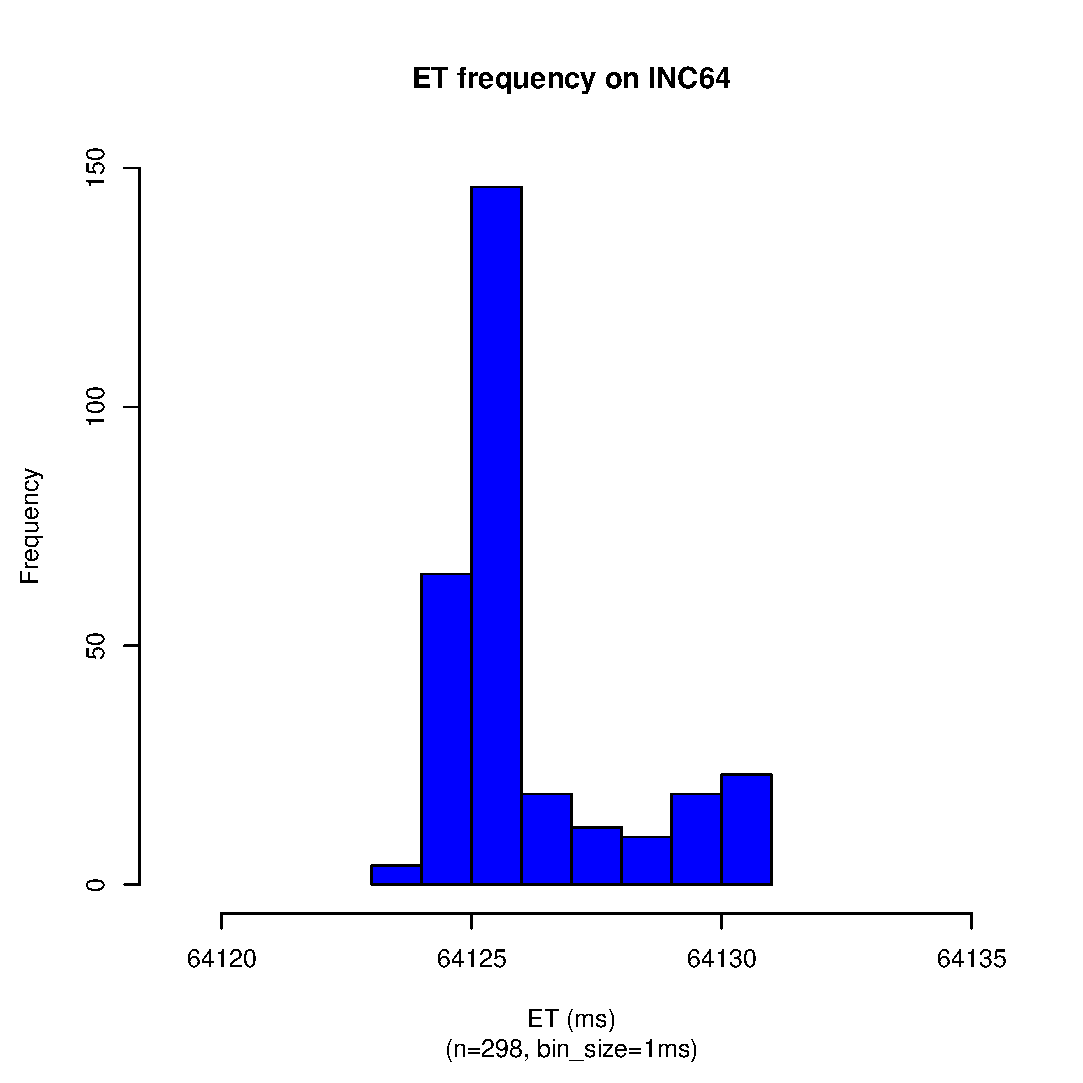
\includegraphics[scale=0.43]{sodb12/64_sec_et_hist_v5.eps}
		\label{fig:s12_inc64_et_hist_v5}
	}
	\subfigure[ET frequency on INC128 on {\tt sodb12}]{
		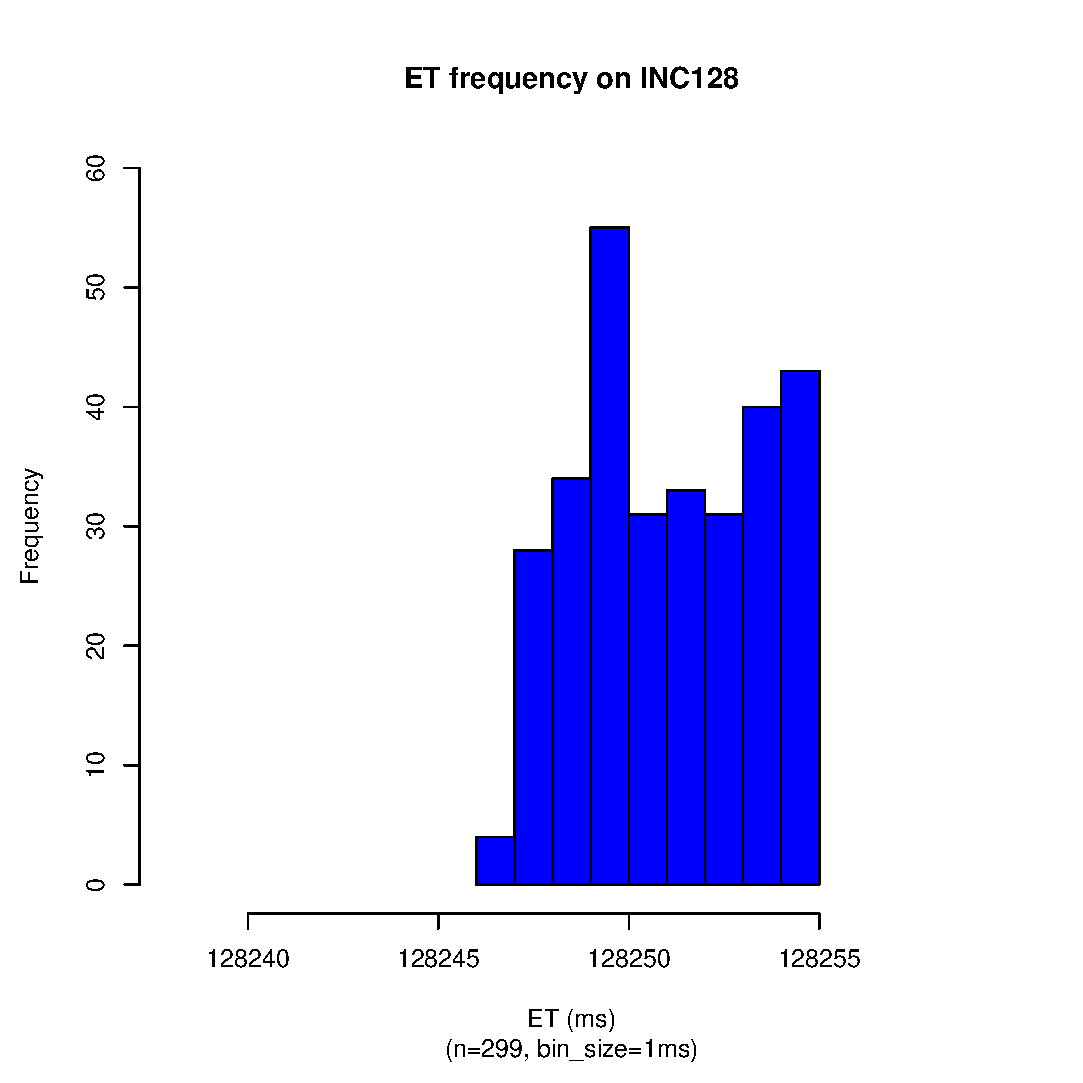
\includegraphics[scale=0.43]{sodb12/128_sec_et_hist_v5.eps}
		\label{fig:s12_inc128_et_hist_v5}
	}
	\caption{ET Histograms of INC16 ... INC128~\label{fig:s12_et_hist2}}
\end{figure}

\newpage

\subsubsection{PT}

\begin{figure}[hp!]
	\centering
	\subfigure[PT frequency on INC1 on {\tt sodb12}]{
		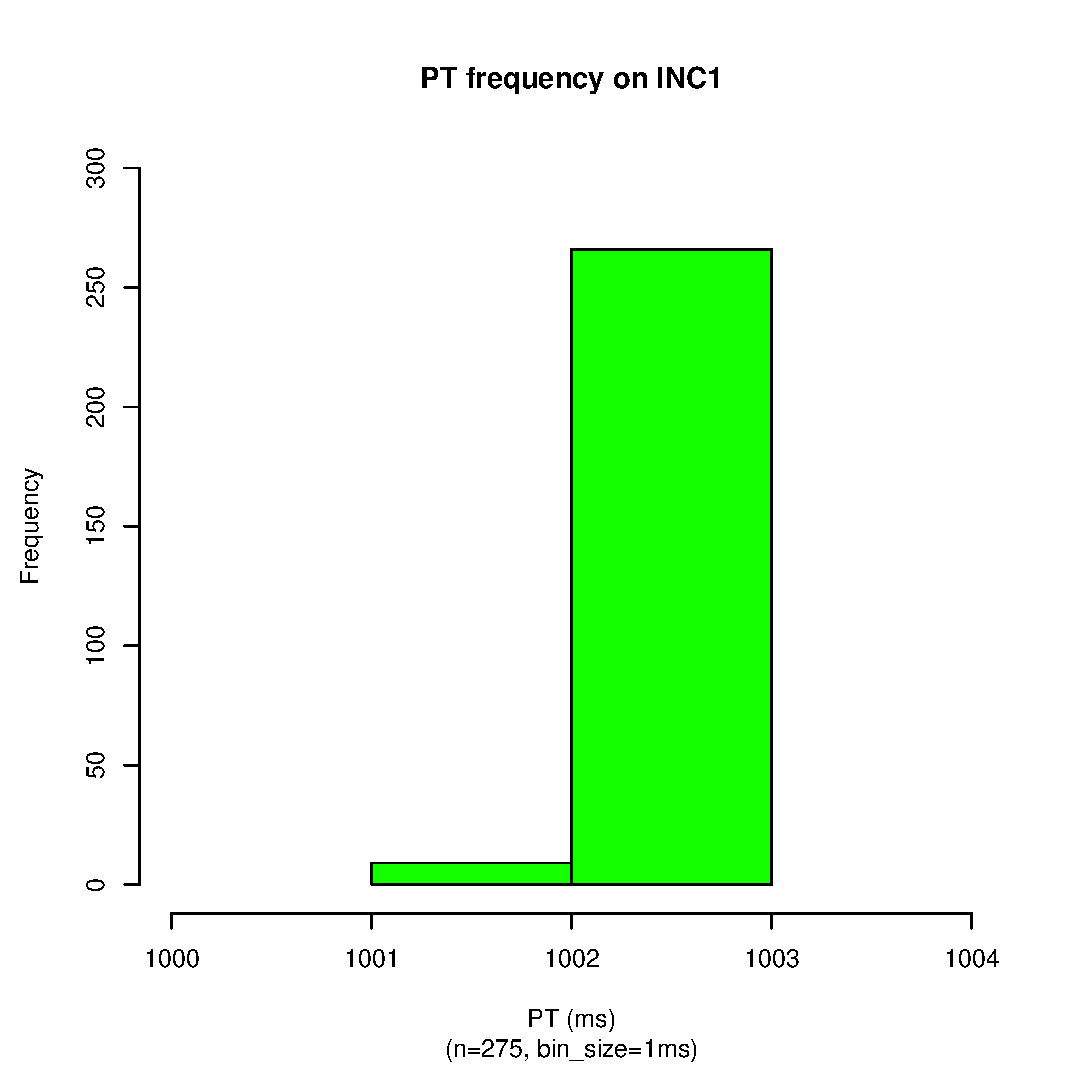
\includegraphics[scale=0.43]{sodb12/1_sec_pt_hist_v5.eps}
		\label{fig:s12_inc1_hist_v5}
	}
	\subfigure[PT frequency on INC2 on {\tt sodb12}]{
		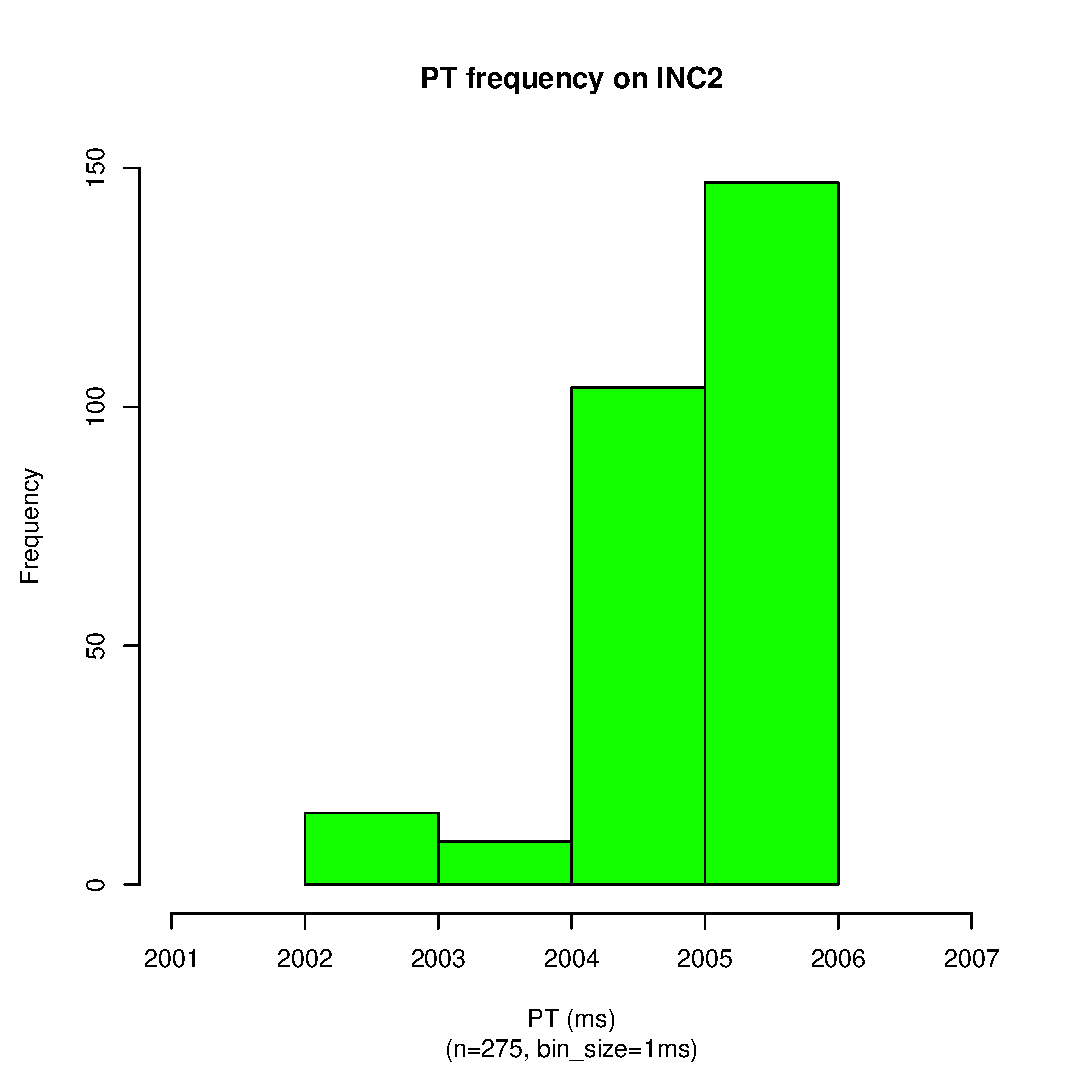
\includegraphics[scale=0.43]{sodb12/2_sec_pt_hist_v5.eps}
		\label{fig:s12_inc2_hist_v5}
	}
	\subfigure[PT frequency on INC4 on {\tt sodb12}]{
		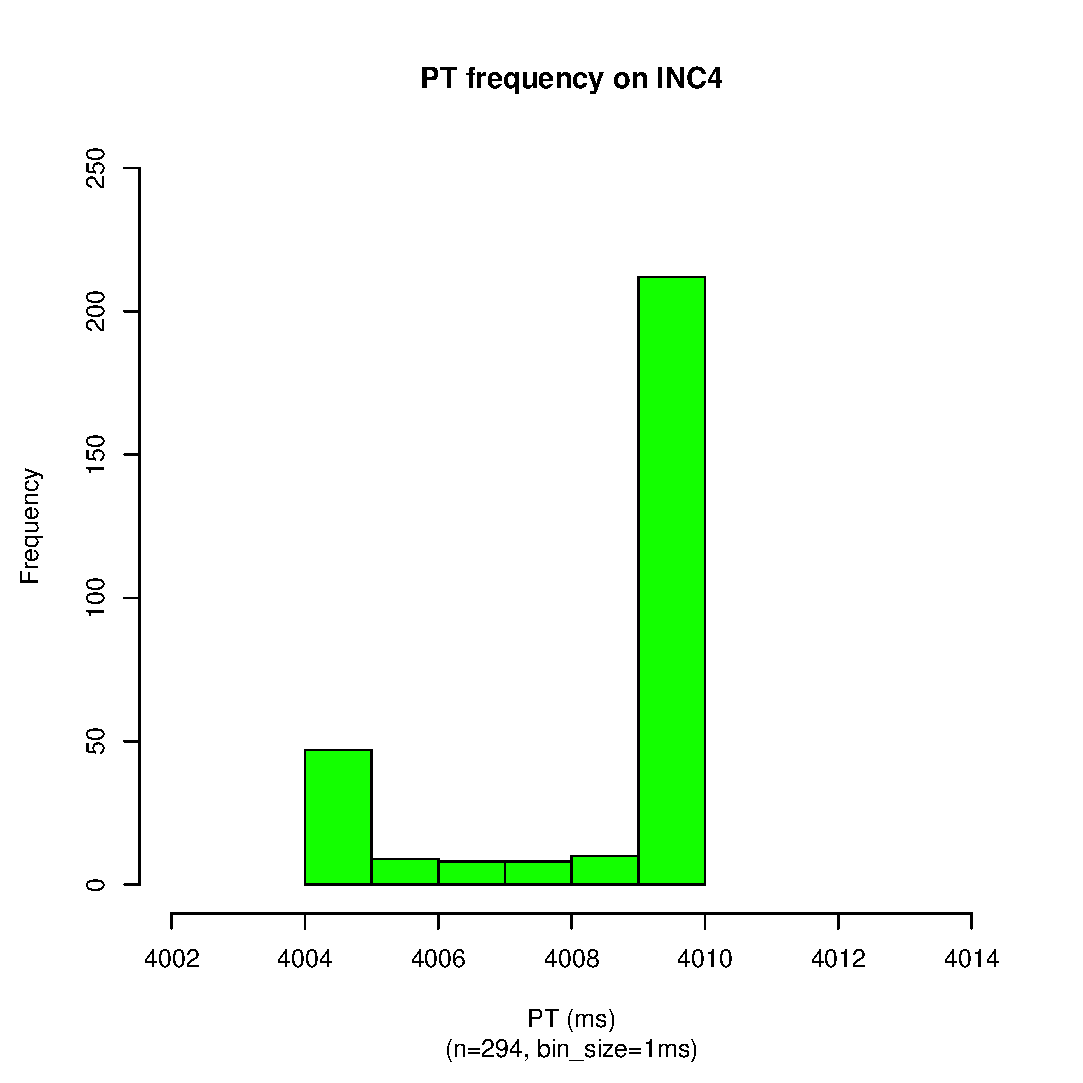
\includegraphics[scale=0.43]{sodb12/4_sec_pt_hist_v5.eps}
		\label{fig:s12_inc4_hist_v5}
	}
	\subfigure[PT frequency on INC8 on {\tt sodb12}]{
		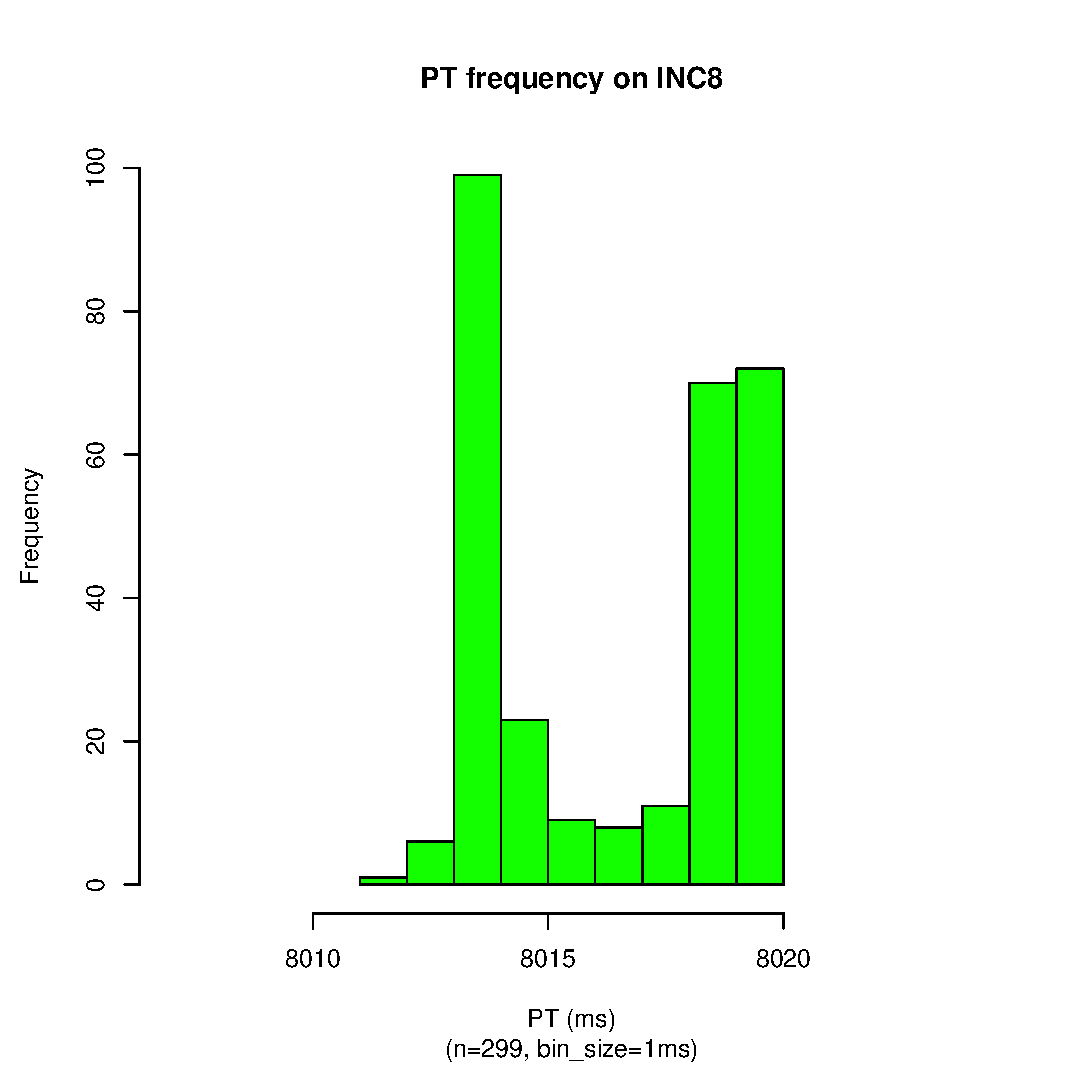
\includegraphics[scale=0.43]{sodb12/8_sec_pt_hist_v5.eps}
		\label{fig:s12_inc8_hist_v5}
	}
	\caption{PT Histograms of INC1 ... INC8~\label{fig:s12_pt_hist1}}
\end{figure}

\begin{figure}[hp!]
	\centering
	\subfigure[PT frequency on INC16 on {\tt sodb12}]{
		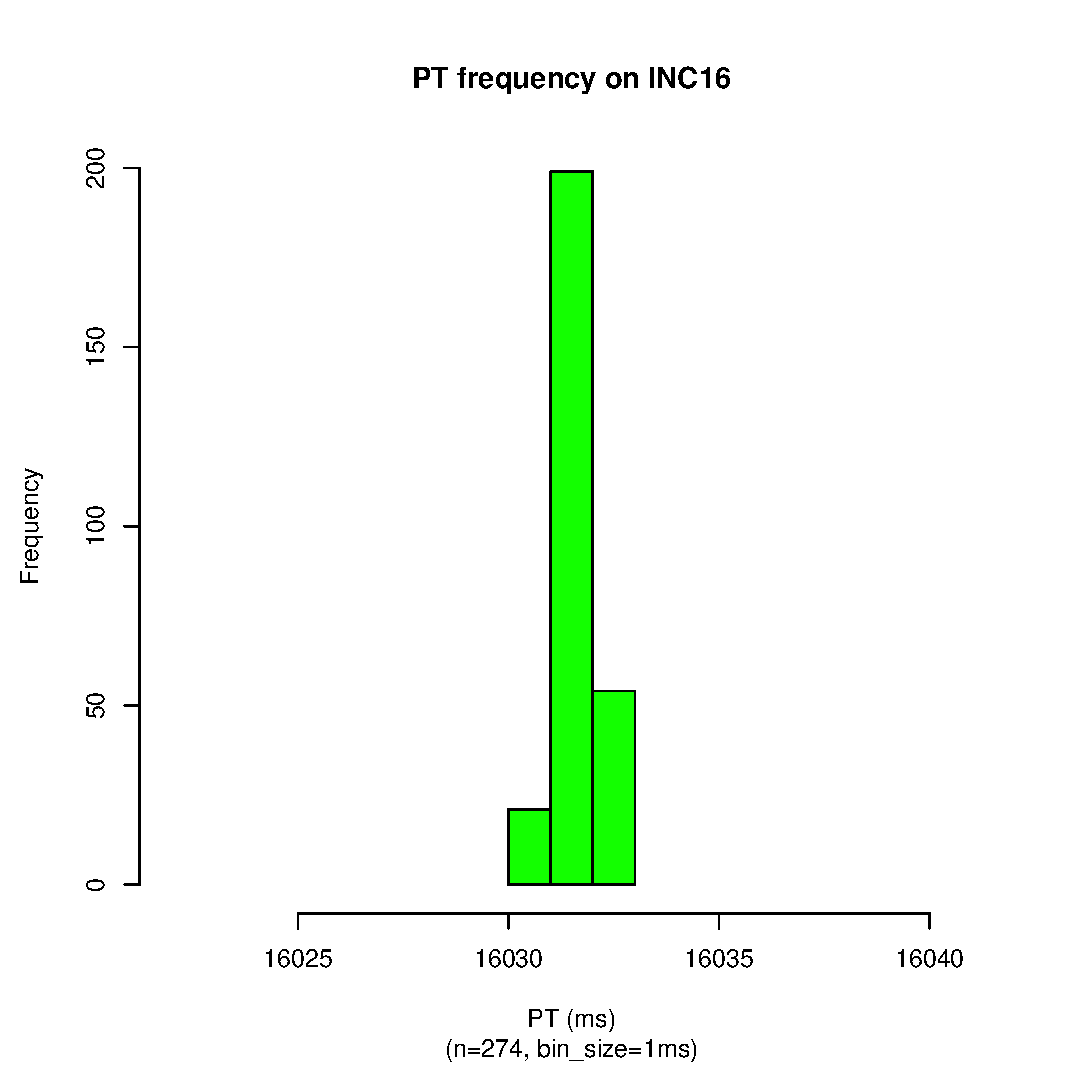
\includegraphics[scale=0.43]{sodb12/16_sec_pt_hist_v5.eps}
		\label{fig:s12_inc16_hist_v5}
	}
	\subfigure[PT frequency on INC32 on {\tt sodb12}]{
		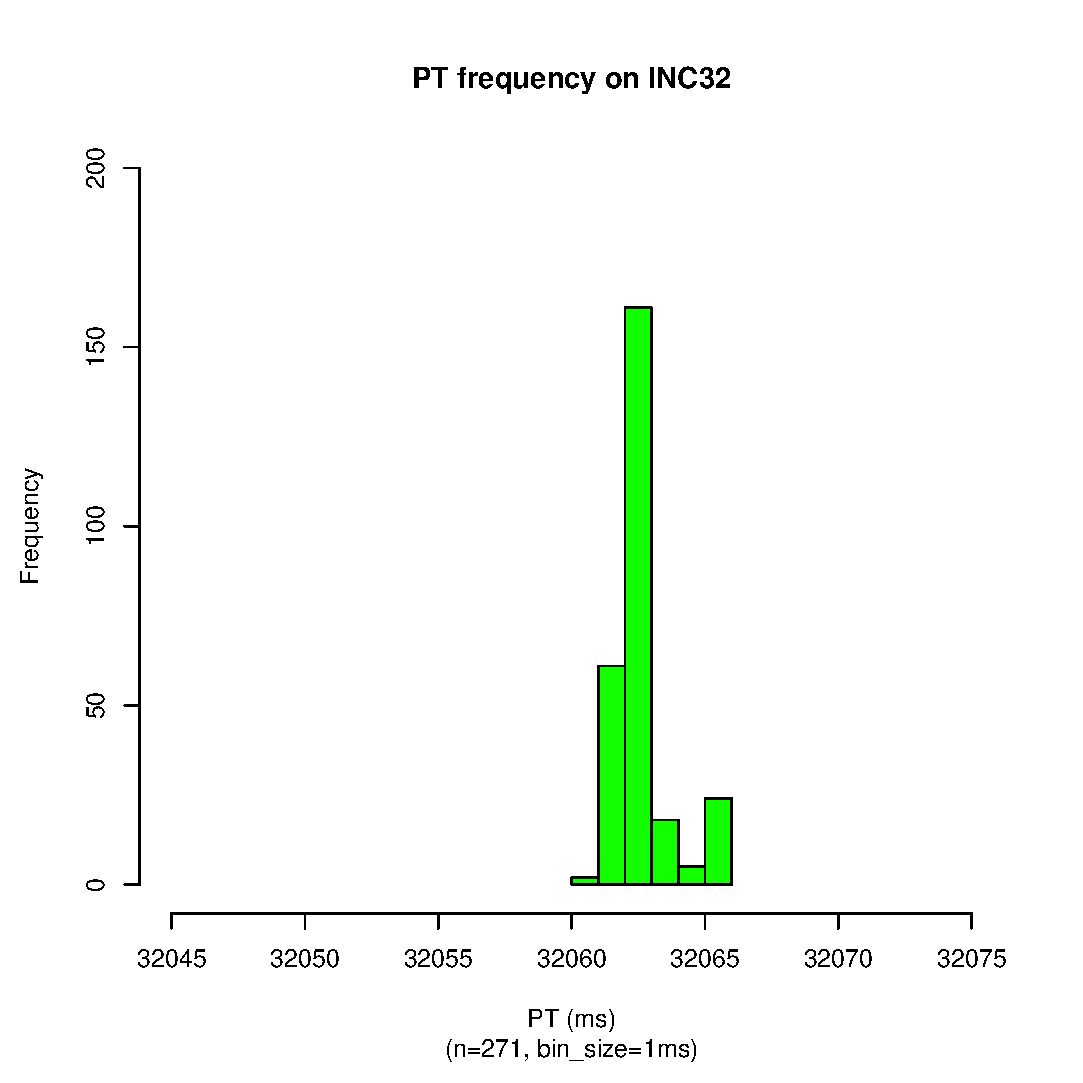
\includegraphics[scale=0.43]{sodb12/32_sec_pt_hist_v5.eps}
		\label{fig:s12_inc32_hist_v5}
	}
	\subfigure[PT frequency on INC64 on {\tt sodb12}]{
		\includegraphics[scale=0.43]{sodb12/64_sec_pt_hist_v5.eps}
		\label{fig:s12_inc64_hist_v5}
	}
	\subfigure[PT frequency on INC128 on {\tt sodb12}]{
		\includegraphics[scale=0.43]{sodb12/128_sec_pt_hist_v5.eps}
		\label{fig:s12_inc128_hist_v5}
	}
	\caption{PT Histograms of INC16 ... INC64~\label{fig:s12_pt_hist2}}
\end{figure}
\newpage

\subsection{{\tt sodb12}~\label{sec:sodb12_hist}} 
This section exhibits histograms on the EMPv5 data obtained on {\tt sodb12}. 
The detailed description of the base data are from Table~\ref{tab:exp_notes}.

\subsubsection{ET}

\begin{figure}[hp!]
	\centering
	\subfigure[ET frequency on INC1 on {\tt sodb12}]{
		\includegraphics[scale=0.43]{sodb12/1_sec_et_hist_v5.eps}
		\label{fig:s12_inc1_et_hist_v5}
	}
	\subfigure[ET frequency on INC2 on {\tt sodb12}]{
		\includegraphics[scale=0.43]{sodb12/2_sec_et_hist_v5.eps}
		\label{fig:s12_inc2_et_hist_v5}
	}
	\subfigure[ET frequency on INC4 on {\tt sodb12}]{
		\includegraphics[scale=0.43]{sodb12/4_sec_et_hist_v5.eps}
		\label{fig:s12_inc4_et_hist_v5}
	}
	\subfigure[ET frequency on INC8 on {\tt sodb12}]{
		\includegraphics[scale=0.43]{sodb12/8_sec_et_hist_v5.eps}
		\label{fig:s12_inc8_et_hist_v5}
	}
	\caption{ET Histograms of INC1 ... INC8~\label{fig:s12_et_hist1}}
\end{figure}

\begin{figure}[hp!]
	\centering
	\subfigure[ET frequency on INC16 on {\tt sodb12}]{
		\includegraphics[scale=0.43]{sodb12/16_sec_et_hist_v5.eps}
		\label{fig:s12_inc16_et_hist_v5}
	}
	\subfigure[ET frequency on INC32 on {\tt sodb12}]{
		\includegraphics[scale=0.43]{sodb12/32_sec_et_hist_v5.eps}
		\label{fig:s12_inc32_et_hist_v5}
	}
	\subfigure[ET frequency on INC64 on {\tt sodb12}]{
		\includegraphics[scale=0.43]{sodb12/64_sec_et_hist_v5.eps}
		\label{fig:s12_inc64_et_hist_v5}
	}
	\subfigure[ET frequency on INC128 on {\tt sodb12}]{
		\includegraphics[scale=0.43]{sodb12/128_sec_et_hist_v5.eps}
		\label{fig:s12_inc128_et_hist_v5}
	}
	\caption{ET Histograms of INC16 ... INC128~\label{fig:s12_et_hist2}}
\end{figure}

\newpage

\subsubsection{PT}

\begin{figure}[hp!]
	\centering
	\subfigure[PT frequency on INC1 on {\tt sodb12}]{
		\includegraphics[scale=0.43]{sodb12/1_sec_pt_hist_v5.eps}
		\label{fig:s12_inc1_hist_v5}
	}
	\subfigure[PT frequency on INC2 on {\tt sodb12}]{
		\includegraphics[scale=0.43]{sodb12/2_sec_pt_hist_v5.eps}
		\label{fig:s12_inc2_hist_v5}
	}
	\subfigure[PT frequency on INC4 on {\tt sodb12}]{
		\includegraphics[scale=0.43]{sodb12/4_sec_pt_hist_v5.eps}
		\label{fig:s12_inc4_hist_v5}
	}
	\subfigure[PT frequency on INC8 on {\tt sodb12}]{
		\includegraphics[scale=0.43]{sodb12/8_sec_pt_hist_v5.eps}
		\label{fig:s12_inc8_hist_v5}
	}
	\caption{PT Histograms of INC1 ... INC8~\label{fig:s12_pt_hist1}}
\end{figure}

\begin{figure}[hp!]
	\centering
	\subfigure[PT frequency on INC16 on {\tt sodb12}]{
		\includegraphics[scale=0.43]{sodb12/16_sec_pt_hist_v5.eps}
		\label{fig:s12_inc16_hist_v5}
	}
	\subfigure[PT frequency on INC32 on {\tt sodb12}]{
		\includegraphics[scale=0.43]{sodb12/32_sec_pt_hist_v5.eps}
		\label{fig:s12_inc32_hist_v5}
	}
	\subfigure[PT frequency on INC64 on {\tt sodb12}]{
		\includegraphics[scale=0.43]{sodb12/64_sec_pt_hist_v5.eps}
		\label{fig:s12_inc64_hist_v5}
	}
	\subfigure[PT frequency on INC128 on {\tt sodb12}]{
		\includegraphics[scale=0.43]{sodb12/128_sec_pt_hist_v5.eps}
		\label{fig:s12_inc128_hist_v5}
	}
	\caption{PT Histograms of INC16 ... INC64~\label{fig:s12_pt_hist2}}
\end{figure}

\clearpage
\newpage

\section{Post Experiments}

We provide a short description of newer experimental runs. 

\paragraph{Experimental Notes:} In the experiments 
we also used four nodes ({\tt sodb8}, {\tt sodb9}, {\tt sodb10}, and {\tt sodb12}) in the same cluster. 
A short summary of the experiments is shown in Table~\ref{tab:exp_notes2}.

%% done
\begin{table}[h]
\begin{center}
\begin{tabular}{|p{4cm}|p{3cm}|p{4cm}|p{4cm}|} \hline
Machine & Task Length & Description & Time Length\\ \hline
{\tt sodb8} (plugged into the {\em upper right} power strip) &  INC16, INC13, and INC17.2 & Runs of 1,000 samples & 2018-03-17 $\sim$2018-03-18\\ \hline
{\tt sodb9}  (plugged into the {\em upper left} power strip) &  IINC16, INC13, and INC17.2 & Runs of 1,000 samples & 2018-03-17 $\sim$2018-03-18\\ \hline
{\tt sodb10} (plugged into the {\em upper left} power strip)  & INC16, INC13, and INC17.2 & Runs of 1,000 samples & 2018-03-17 $\sim$2018-03-18\\ \hline
{\tt sodb12} (plugged into the {\em upper right} power strip) & INC16, INC13, and INC17.2 & Runs of 1,000 samples & 2018-03-17 $\sim$2018-03-18\\ \hline
\end{tabular}
\end{center}
\vspace{-.2in}
\caption{Detailed description of INC data used for histograms\label{tab:exp_notes2}}
\end{table}

\subsection{Inter-Machine Homogeneity~\label{sec:diff_machine}} 

In this section we check if the use of different machines affects the distribution of execution (process) times on the same program. 
In other words, we examine {\em inter-machine repeatability}. For this examination, we use a nested for loop program, here termed INC, 
with different task lengths: 16 seconds, 13 seconds, and 17.2 seconds, each termed {\em INC16}, {\em INC13}, and {\em INC17.2}, respectively. 

Figures~\ref{fig:dm_1}, ~\ref{fig:dm_2}, and ~\ref{fig:dm_3} display the process time (PT) histograms on INC16, INC13, and INC17.2 run on our machines (from {\tt sodb8} to {\tt sodb12}), respectively. Based on these figures, we conclude that we should stick to one machine  for consistency, and {\tt sodb9} should be chosen in a sense that the data measured there consistently reveals a distinct binormal pattern.

\begin{figure}[h]
	\centering
	\subfigure[PT frequency on INC16]{
		\includegraphics[scale=0.43]{newer_exp/sodb8_INC16_0_dist.eps}
		\label{fig:s8_inc16_dist}
	}	
	\subfigure[PT frequency on INC16]{
		\includegraphics[scale=0.43]{newer_exp/sodb9_INC16_0_dist.eps}
		\label{fig:s9_inc16_dist}
	}
	\subfigure[PT frequency on INC16]{
		\includegraphics[scale=0.43]{newer_exp/sodb10_INC16_0_dist.eps}
		\label{fig:s10_inc16_dist}
	}	
	\subfigure[PT frequency on INC16]{
		\includegraphics[scale=0.43]{newer_exp/sodb12_INC16_0_dist.eps}
		\label{fig:s12_inc16_dist}
	}
	\caption{PT Histograms on INC16~\label{fig:dm_1}}
\end{figure}


\newpage
\clearpage

\begin{figure}[h]
	\centering
	\subfigure[PT frequency on INC13]{
		\includegraphics[scale=0.43]{newer_exp/sodb8_INC13_0_dist.eps}
		\label{fig:s8_inc13_dist}
	}	
	\subfigure[PT frequency on INC13]{
		\includegraphics[scale=0.43]{newer_exp/sodb9_INC13_0_dist.eps}
		\label{fig:s9_inc13_dist}
	}
	\subfigure[PT frequency on INC13]{
		\includegraphics[scale=0.43]{newer_exp/sodb10_INC13_0_dist.eps}
		\label{fig:s10_inc13_dist}
	}	
	\subfigure[PT frequency on INC13]{
		\includegraphics[scale=0.43]{newer_exp/sodb12_INC13_0_dist.eps}
		\label{fig:s12_inc13_dist}
	}
	\caption{PT Histograms on INC13~\label{fig:dm_2}}
\end{figure}

\newpage
\clearpage

\begin{figure}[h]
	\centering
	\subfigure[PT frequency on INC17.2]{
		\includegraphics[scale=0.43]{newer_exp/sodb8_INC17_2_dist.eps}
		\label{fig:s8_inc17_2_dist}
	}	
	\subfigure[PT frequency on INC17.2]{
		\includegraphics[scale=0.43]{newer_exp/sodb9_INC17_2_dist.eps}
		\label{fig:s9_inc17_2_dist}
	}
	\subfigure[PT frequency on INC17.2]{
		\includegraphics[scale=0.43]{newer_exp/sodb10_INC17_2_dist.eps}
		\label{fig:s10_inc17_2_dist}
	}	
	\subfigure[PT frequency on INC17.2]{
		\includegraphics[scale=0.43]{newer_exp/sodb12_INC17_2_dist.eps}
		\label{fig:s12_inc17_2_dist}
	}
	\caption{PT Histograms on INC17.2~\label{fig:dm_3}}
\end{figure}

\newpage
\clearpage

\subsection{Intra-Machine Homogeneity~\label{sec:intra_machine}} 

A short description of the runs we used for this experiment are exhibited in Table~\ref{tab:exp_notes3}.

%\paragraph{Experimental Notes:} In the experiments 
%we used only {\tt sodb9}. A short summary of the experiments is shown in Table~\ref{tab:exp_notes3}.
%\vspace{-.3in}
%% done
\begin{table}[h]
\begin{center}
\begin{tabular}{|p{4cm}|p{3cm}|p{4cm}|p{4cm}|} \hline
Machine & Task Length & Description & Time Length\\ \hline
{\tt sodb9}  (plugged into the {\em upper left} power strip) &  INC1$\sim$INC128 & Runs of 1,000 samples & 2018-04-28 $\sim$2018-04-30\\ \hline
\end{tabular}
\end{center}
\vspace{-.2in}
\caption{Detailed description of INC data used for histograms\label{tab:exp_notes3}}
\end{table}

%\newpage
%\clearpage

\begin{figure}[H]
	\centering
	\subfigure[PT frequency on INC1 on {\tt sodb9}]{
		\includegraphics[scale=0.43]{new_INC_data_s9/s9_INC1_dist.eps}
		\label{fig:s9_inc1_dist}
	}
	\subfigure[PT frequency on INC2 on {\tt sodb9}]{
		\includegraphics[scale=0.43]{new_INC_data_s9/s9_INC2_dist.eps}
		\label{fig:s9_inc2_dist}
	}
	\subfigure[PT frequency on INC4 on {\tt sodb9}]{
		\includegraphics[scale=0.43]{new_INC_data_s9/s9_INC4_dist.eps}
		\label{fig:s9_inc4_dist}
	}
	\subfigure[PT frequency on INC8 on {\tt sodb9}]{
		\includegraphics[scale=0.43]{new_INC_data_s9/s9_INC8_dist.eps}
		\label{fig:s9_inc8_dist}
	}
	\caption{PT Histograms on INC1$\sim$INC8\label{fig:new_data1}}
\end{figure}

\newpage
\clearpage

\begin{figure}[h]
	\centering
	\subfigure[PT frequency on INC16 on {\tt sodb9}]{
		\includegraphics[scale=0.43]{new_INC_data_s9/s9_INC16_dist.eps}
		\label{fig:s9_inc16_dist2}
	}
	\subfigure[PT frequency on INC32 on {\tt sodb9}]{
		\includegraphics[scale=0.43]{new_INC_data_s9/s9_INC32_dist.eps}
		\label{fig:s9_inc32_dist}
	}
	\subfigure[PT frequency on INC64 on {\tt sodb9}]{
		\includegraphics[scale=0.43]{new_INC_data_s9/s9_INC64_dist.eps}
		\label{fig:s9_inc64_dist}
	}
	\subfigure[PT frequency on INC128 on {\tt sodb9}]{
		\includegraphics[scale=0.43]{new_INC_data_s9/s9_INC128_dist.eps}
		\label{fig:s9_inc128_dist}
	}
	\caption{PT Histograms on INC16$\sim$INC128\label{fig:new_data2}}
\end{figure}

\newpage
\clearpage
\subsection{Power Strip Influence~\label{sec:sodb8}} 

A short description of the runs we used for this experiment are exhibited in Table~\ref{tab:exp_notes4}.

\begin{table}[h]
\begin{center}
\begin{tabular}{|p{4cm}|p{3cm}|p{4cm}|p{4cm}|} \hline
Machine & Task Length & Description & Time Length\\ \hline
{\tt sodb8}  (plugged into the {\em bottom left} power strip) &  INC13 & Runs of 1,000 samples & 2018-03-17 $\sim$2018-03-18\\ \hline
{\tt sodb8}  (plugged into the {\em upper right} power strip) &  INC13 & Runs of 1,000 samples & 2018-04-28 $\sim$2018-04-30\\ \hline
\end{tabular}
\end{center}
\vspace{-.2in}
\caption{Detailed description of INC data used for histograms\label{tab:exp_notes4}}
\end{table}

\begin{figure}[H]
	\centering
	\subfigure[PT frequency on INC13 on {\tt sodb8}  (plugged into the {\em bottom left} power strip) (copied from Fig.~\ref{fig:s8_inc13_dist})]{
		\includegraphics[scale=0.43]{newer_exp/sodb8_INC13_0_dist.eps}
		\label{fig:s8_inc13_dist_before}
	}
	\subfigure[PT frequency on INC13 on {\tt sodb8}  (plugged into the {\em upper right} power strip)]{
		\includegraphics[scale=0.43]{new_INC_data_s9/s8_INC13_dist.eps}
		\label{fig:s8_inc13_dist_after}
	}
	\caption{PT Histograms on INC13 on {\tt sodb8} Before and After Power Strip Relocation\label{fig:power_strip}}
\end{figure}

\newpage
\clearpage

\subsection{Investigation of Daemons' Influence on Program Time Distribution Regarding Machine Dependence~\label{sec:daemon_impact}} 

For the same task length, or INC16, 
I examined in each of the four runs a few iterations at which more than three daemons (except INC and proc monitor processes) that had positive PT were captured.  
From Table~\ref{tab:daemon}, I suspect that PT distribution seems most likely to be affected by two facts: {\it how longer the same daemon ran than usual}, and {\it how many different daemon processes appeared and how long it ran}.

\begin{table}[htp!]
\centering
{
 \begin{tabular}{|p{1.5cm}|p{2cm}|p{12.5cm}|} \hline
Machine Name & Iteration \# & Process Name (id, PT(msec))\\ \hline
{\tt sodb8}  & 174 & {\tt java} ({\tt 2349}, 15), {\tt java} ({\tt 2335}, 2),  {\tt md127\_raid1} ({\tt 457}, 1), {\tt kslowd000} ({\tt 166}, 1), {\tt kslowd001} ({\tt 167}, 1) \\ \cline{2-3}
 					& 278 & {\tt java} ({\tt 2877}, 16), {\tt java} ({\tt 2335}, 2),  {\tt kslowd000} ({\tt 166}, 1), {\tt kslowd001} ({\tt 167}, 1) \\ \cline{2-3}
			  &  486 & {\tt java} ({\tt 3190}, 21), {\tt java} ({\tt 2335}, 2),  {\tt md127\_raid1} ({\tt 457}, 1), {\tt kslowd000} ({\tt 166}, 1)\\ \cline{2-3}
				  &  526 & {\tt md127\_raid1} ({\tt 457}, 1), {\tt kslowd000} ({\tt 166}, 1), {\tt kslowd001} ({\tt 167}, 1), {\tt jbd2/md127-8} ({\tt 470}, 1)\\ \cline{2-3}
				  &  555 & {\tt java} ({\tt 3815}, 8), {\tt java} ({\tt 2335}, 2), {\tt kslowd000} ({\tt 166}, 1), {\tt kslowd001} ({\tt 167}, 1)\\ \hline
{\tt sodb9}  & 105 & {\tt java} ({\tt 6634}, 16), {\tt java} ({\tt 6621}, 2),  {\tt kslowd000} ({\tt 166}, 1), {\tt kslowd001} ({\tt 167}, 1) \\ \cline{2-3}
				  & 175 & {\tt java} ({\tt 6942}, 7), {\tt java} ({\tt 6621}, 2),  {\tt kslowd000} ({\tt 166}, 1), {\tt kslowd001} ({\tt 167}, 1) \\ \cline{2-3}
				  & 245 & {\tt java} ({\tt 7259}, 6), {\tt java} ({\tt 6621}, 2),  {\tt kslowd000} ({\tt 166}, 1), {\tt kslowd001} ({\tt 167}, 1) \\ \cline{2-3}
				  & 280 & {\tt java} ({\tt 7365}, 3), {\tt java} ({\tt 6621}, 2),  {\tt kslowd000} ({\tt 166}, 1), {\tt kslowd001} ({\tt 167}, 1) \\ \cline{2-3}
				  & 350 & {\tt java} ({\tt 7577}, 3), {\tt java} ({\tt 6621}, 2),  {\tt kslowd000} ({\tt 166}, 1), {\tt kslowd001} ({\tt 167}, 1) \\ \cline{2-3}
				  & 420 & {\tt java} ({\tt 7683}, 3), {\tt java} ({\tt 6621}, 2),  {\tt kslowd000} ({\tt 166}, 1), {\tt kslowd001} ({\tt 167}, 1) \\ \cline{2-3}
				  & 490 & {\tt java} ({\tt 7894}, 4), {\tt java} ({\tt 6621}, 2),  {\tt kslowd000} ({\tt 166}, 1), {\tt kslowd001} ({\tt 167}, 1) \\ \hline
{\tt sodb10}  & 105 & {\tt java} ({\tt 28394}, 14), {\tt java} ({\tt 28381}, 2),  {\tt kslowd000} ({\tt 166}, 1), {\tt kslowd001} ({\tt 167}, 1) \\ \cline{2-3}
					 & 314 & {\tt java} ({\tt 28702}, 18), {\tt java} ({\tt 28381}, 2),  {\tt md127\_raid1} ({\tt 455}, 1),  {\tt kslowd001} ({\tt 167}, 1) \\ \hline
 {\tt sodb12}  & 280 &  {\tt kslowd001} ({\tt 167}, 154),  {\tt kslowd000} ({\tt 166}, 150), {\tt java} ({\tt 14820}, 37), {\tt java} ({\tt 14807}, 2) \\ \cline{2-3}
	& 311 &  {\tt kslowd000} ({\tt 166}, 154),  {\tt kslowd001} ({\tt 167}, 153), {\tt java} ({\tt 14807}, 2), {\tt java} ({\tt 15653}, 1), {\tt khugepaged} ({\tt 30}, 1)\\ \cline{2-3}		& 373 &  {\tt kslowd000} ({\tt 166}, 154),  {\tt kslowd001} ({\tt 167}, 152), {\tt java} ({\tt 14807}, 2), {\tt java} ({\tt 15747}, 2)\\ \cline{2-3}
& 435 &  {\tt kslowd000} ({\tt 166}, 154),  {\tt kslowd001} ({\tt 167}, 153), {\tt java} ({\tt 15934}, 6), {\tt java} ({\tt 14807}, 2)\\ \cline{2-3}
& 466 &  {\tt kslowd000} ({\tt 166}, 152), {\tt java} ({\tt 16121}, 6), {\tt java} ({\tt 14807}, 2), {\tt kblockd/0} ({\tt 16}, 1)\\ \cline{2-3}
 \hline
 \end{tabular}
  }
 \caption{Some daemon processes captured across different machines~\label{tab:daemon}}
\end{table}

Similarly, we looked at the data from INC128 on {\tt sodb12}. 

\begin{table}[h]
\begin{center}
\begin{tabular}{|p{4cm}|p{3cm}|p{4cm}|p{4cm}|} \hline
Machine & Task Length & Description & Time Length\\ \hline
{\tt sodb12}  (plugged into the {\em upper right} power strip) &  INC128 & Runs of 1,000 samples & 2017-02-09$\sim$2017-02-10\\ \hline
\end{tabular}
\end{center}
\vspace{-.2in}
\caption{Detailed description of the INC128 data\label{tab:exp_notes5}}
\end{table}


Table~\ref{tab:daemon2} shows a list of daemon processes observed at some iterations for which more than three daemons revealed positive PT while the INC128 program was run.
\begin{table}[htp!]
\centering
{
 \begin{tabular}{|p{1.5cm}|p{2cm}|p{12.5cm}|} \hline
Machine Name & Iteration \# & Process Name (id, PT(msec))\\ \hline
 {\tt sodb12}  & 33 & {\tt flush-9:0} ({\tt 25187}, 1), {\tt java} ({\tt 304}, 1), {\tt java} ({\tt 32627}, 3), {\tt md0\_raid1} ({\tt 484}, 1) \\ \cline{2-3}
					  & 138  & {\tt flush-9:0} ({\tt 25187}, 1), {\tt java} ({\tt 734}, 1), {\tt java} ({\tt 32627}, 3), {\tt md0\_raid1} ({\tt 484}, 1)  \\ \cline{2-3}
					  & 181 & {\tt flush-9:0} ({\tt 25187}, 1), {\tt java} ({\tt 908}, 1), {\tt java} ({\tt 32627}, 3), {\tt jbd2/md0-8} ({\tt 497}, 1) \\ \cline{2-3}
				     & 228 &  {\tt flush-9:0} ({\tt 25187}, 1), {\tt java} ({\tt 1099}, 1), {\tt java} ({\tt 32627}, 3), {\tt md0\_raid1} ({\tt 484}, 1)\\ \cline{2-3}
 \hline
 \end{tabular}
  }
 \caption{Some daemon processes captured at some iterations of INC128~\label{tab:daemon2}}
\end{table}

Table~\ref{tab:exp_notes6} gives a background description of what environment 
was set for running the MATR8K program.

\begin{table}[h]
\begin{center}
\begin{tabular}{|p{4cm}|p{3cm}|p{4cm}|p{4cm}|} \hline
Machine & Task Length & Description & Time Length\\ \hline
{\tt sodb12} (plugged into {\em the upper right} power strip) & MATR8K& Runs of 300 samples & 2018-03-02 $\sim$2018-03-12 \\ \hline
\end{tabular}
\end{center}
\vspace{-.2in}
\caption{Detailed description of the MATR8K data\label{tab:exp_notes6}}
\end{table}

Table~\ref{tab:daemon3} shows a list of daemon processes 
observed at some iterations for which a number of daemons revealed positive PT while the MATR8K program was run.
\begin{table}[htp!]
\centering
{ %{\tt bash} ({\tt 17403}, 1), {\tt bash} ({\tt 17400}, 7),  
 \begin{tabular}{|p{1.5cm}|p{2cm}|p{12.5cm}|} \hline
Machine Name & Iteration \# & Process Name (id, PT(msec))\\ \hline
 {\tt sodb12}  & 
 36 & ({\tt MATR8K} ({\tt 17244}, 2183274),{\tt proc\_monitor} ({\tt 14166}, 200)), 
 {\tt kslowd001} ({\tt 167}, 16959),  {\tt kslowd000} ({\tt 166}, 16707), 
 {\tt md0\_raid1 } ({\tt 482}, 19),  {\tt sshd} ({\tt 17398}, 18), {\tt bash}  ({\tt 17400}, 7),  
 {\tt flush-9:0} ({\tt 718}, 3), {\tt java} ({\tt 17234}, 2), {\tt kblockd/0} ({\tt 16}, 2), 
 {\tt grep} ({\tt 17406}, 1), {\tt sshd} ({\tt 17399}, 1), 
 {\tt events/0} ({\tt 7}, 1), {\tt bash} ({\tt 17403}, 1))\\ \cline{2-3} 
&  119 & ({\tt MATR8K} ({\tt 17244}, 2183217),{\tt proc\_monitor} ({\tt 14166}, 204))
 {\tt kslowd001} ({\tt 167}, 16784),  {\tt kslowd000} ({\tt 166}, 16839), 
 {\tt md0\_raid1 } ({\tt 482}, 16),  {\tt  jbd2/md0-8} ({\tt 495}, 13), 
 {\tt sshd} ({\tt 17773}, 7), {\tt sshd} ({\tt 17771}, 7), 
 {\tt kblockd/0} ({\tt 16}, 4),  {\tt events/0} ({\tt 7}, 3), 
 {\tt flush-9:0} ({\tt 718}, 3), {\tt java} ({\tt 17234}, 2), 
 {\tt sshd} ({\tt 17772}, 2),  {\tt sshd} ({\tt 2148}, 1), 
 {\tt java} ({\tt 17768}, 2), {\tt sshd} ({\tt 17774}, 1)\\ \cline{2-3}
 \hline
 \end{tabular}
  }
 \caption{Some daemon processes captured at some iterations of MATR8K~\label{tab:daemon3}}
\end{table}


%\newpage

\section{Conclusion}
My recommendation is to avoid {\tt sodb8} and to use the rest of 
the SoDB nodes for the rest of our experiments. Further investigation is 
needed to examine why the experiment results on {\tt sodb8} are different 
than those of the other nodes. 


\end{document}